% !TeX program = xelatex
% !TeX encoding = UTF-8
\documentclass[12pt,openany,oneside]{book}

\usepackage[a4paper,top=23mm,bottom=25mm,left=25mm,right=25mm,headheight=17pt]{geometry}
\usepackage{amsmath,amssymb,amsfonts,mathtools,bm}
\usepackage{amsthm}
\usepackage{booktabs,longtable,array,multirow,tabularx}
\usepackage{graphicx}
\graphicspath{{figures/}}
\usepackage{xcolor}
\usepackage{tikz}
\usetikzlibrary{arrows.meta,positioning,calc,fit,shapes.geometric,decorations.pathreplacing,matrix,patterns}
\usepackage[most]{tcolorbox}
\usepackage{enumitem}
\usepackage{listings}
\usepackage{caption}
\usepackage{subcaption}
\usepackage{float}
\usepackage{fancyhdr}
\usepackage{titlesec}
\usepackage{setspace}
\usepackage{microtype}
\usepackage{hyperref}
\usepackage{xepersian}

\settextfont[Scale=1.08]{Amiri}
\setlatintextfont{DejaVu Serif}
\setmonofont{DejaVu Sans Mono}
\setdigitfont{Amiri}

\definecolor{DeepBlue}{HTML}{163A5F}
\definecolor{Accent}{HTML}{B34B35}
\definecolor{SoftBlue}{HTML}{EAF2F8}
\definecolor{SoftGold}{HTML}{FFF6DF}
\definecolor{SoftGreen}{HTML}{EAF7EF}
\definecolor{SoftRed}{HTML}{FCEDEC}
\definecolor{SoftGray}{HTML}{F4F5F6}
\definecolor{CodeGray}{HTML}{F7F7F7}

\hypersetup{
  colorlinks=true,
  linkcolor=DeepBlue,
  citecolor=Accent,
  urlcolor=Accent,
  pdftitle={پردازش تصویر در دهه آینده ـ فصل سوم: سامانه‌های خطی، فوریه و نمایش چندمقیاسی},
  pdfauthor={جزوه درس کارشناسی ارشد}
}

\setstretch{1.22}
\setlength{\parskip}{0.35em}
\setlength{\parindent}{1.3em}
\setlist[itemize]{itemsep=0.25em,topsep=0.35em}
\setlist[enumerate]{itemsep=0.25em,topsep=0.35em}

\pagestyle{fancy}
\fancyhf{}
\fancyhead[R]{\small\thepage}
\fancyhead[L]{\small\nouppercase{\leftmark}}
\renewcommand{\headrulewidth}{0.4pt}

\titleformat{\chapter}[display]
  {\normalfont\huge\bfseries\color{DeepBlue}}
  {\filleft\Large فصل \thechapter}
  {8pt}
  {\filright}
\titleformat{\section}{\Large\bfseries\color{DeepBlue}}{\thesection}{0.7em}{}
\titleformat{\subsection}{\large\bfseries\color{Accent}}{\thesubsection}{0.7em}{}

\newtheorem{definition}{تعریف}[chapter]
\newtheorem{theorem}{قضیه}[chapter]
\newtheorem{proposition}{گزاره}[chapter]
\newtheorem{lemma}{لم}[chapter]
\newtheorem{example}{مثال}[chapter]
\newtheorem{remark}{نکته}[chapter]
\newtheorem{corollary}{نتیجه}[chapter]
\renewcommand{\proofname}{اثبات}

\newtcolorbox{learningbox}{
  colback=SoftBlue,colframe=DeepBlue,title=اهداف یادگیری,
  fonttitle=\bfseries,breakable,enhanced}
\newtcolorbox{keybox}[1][]{
  colback=SoftGold,colframe=Accent,title={#1},
  fonttitle=\bfseries,breakable,enhanced}
\newtcolorbox{futurebox}{
  colback=SoftGreen,colframe=green!50!black,title=پل به دهه آینده,
  fonttitle=\bfseries,breakable,enhanced}
\newtcolorbox{warningbox}{
  colback=SoftRed,colframe=red!65!black,title=خطای رایج,
  fonttitle=\bfseries,breakable,enhanced}
\newtcolorbox{workshopbox}[1][]{
  colback=SoftGray,colframe=black!55,title={کارگاه خانگی پردازش تصویر: #1},
  fonttitle=\bfseries,breakable,enhanced}
\newtcolorbox{researchbox}[1][]{
  colback=white,colframe=purple!65!black,title={خواندن مقاله و استاندارد: #1},
  fonttitle=\bfseries,breakable,enhanced}
\newtcolorbox{videobox}{
  colback=white,colframe=DeepBlue,title=تقسیم پیشنهادی ویدئوهای ۱۵ دقیقه‌ای,
  fonttitle=\bfseries,breakable,enhanced}
\newtcolorbox{proofbox}[1][]{
  colback=white,colframe=DeepBlue!65,title={مسیر اثبات: #1},
  fonttitle=\bfseries,breakable,enhanced}

\newcommand{\R}{\mathbb{R}}
\newcommand{\C}{\mathbb{C}}
\newcommand{\N}{\mathbb{N}}
\newcommand{\Z}{\mathbb{Z}}
\newcommand{\E}{\mathbb{E}}
\newcommand{\Var}{\operatorname{Var}}
\newcommand{\Cov}{\operatorname{Cov}}
\newcommand{\Prob}{\mathbb{P}}
\newcommand{\norm}[1]{\left\lVert #1\right\rVert}
\newcommand{\abs}[1]{\left\lvert #1\right\rvert}
\newcommand{\inner}[2]{\left\langle #1,#2\right\rangle}
\newcommand{\trans}{^{\mathsf T}}
\newcommand{\herm}{^{\mathsf H}}
\newcommand{\lrterm}[1]{\lr{#1}}
\newcommand{\vect}[1]{\bm{#1}}
\newcommand{\op}[1]{\mathcal{#1}}
\newcommand{\FT}{\mathcal{F}}
\newcommand{\sinc}{\operatorname{sinc}}
\newcommand{\diag}{\operatorname{diag}}
\newcommand{\argmin}{\operatorname*{arg\,min}}
\newcommand{\supp}{\operatorname{supp}}
\newcommand{\rank}{\operatorname{rank}}
\newcommand{\trace}{\operatorname{tr}}
\newcommand{\cond}{\operatorname{cond}}
\newcommand{\PSNR}{\operatorname{PSNR}}
\newcommand{\SSIM}{\operatorname{SSIM}}
\newcommand{\DFT}{\operatorname{DFT}}
\newcommand{\FFT}{\operatorname{FFT}}
\newcommand{\rect}{\operatorname{rect}}
\newcommand{\sgn}{\operatorname{sgn}}
\newcommand{\esssup}{\operatorname*{ess\,sup}}

\lstset{
  language=Python,
  basicstyle=\small\ttfamily,
  backgroundcolor=\color{CodeGray},
  frame=single,
  rulecolor=\color{black!25},
  numbers=left,
  numberstyle=\tiny,
  breaklines=true,
  showstringspaces=false,
  keywordstyle=\bfseries,
  commentstyle=\itshape,
  tabsize=4
}

% Auto-generated by generate_ch03_figures.py
\newcommand{\chthreeBoundaryConstantRmse}{0.135416}
\newcommand{\chthreeBoundaryReflectRmse}{0.00114405}
\newcommand{\chthreeBoundaryWrapRmse}{0.0912732}
\newcommand{\chthreeDftOffdiagRatio}{9.68639e-15}
\newcommand{\chthreeExtremaFinal}{13}
\newcommand{\chthreeExtremaInitial}{235}
\newcommand{\chthreeFftSpeedupNFiveOneTwo}{12960.8}
\newcommand{\chthreeFftVsZeroSpatialRelLTwo}{6.36092e-16}
\newcommand{\chthreeFftZeroSeconds}{0.0109315}
\newcommand{\chthreeFourierHighAmpFinal}{0.34921}
\newcommand{\chthreeFourierLossFinal}{6.51075e-05}
\newcommand{\chthreeGibbsOvershootFcZeroZeroThree}{0.0894937}
\newcommand{\chthreeGibbsOvershootFcZeroZeroEight}{0.0896774}
\newcommand{\chthreeGibbsOvershootFcZeroOneSix}{0.0859501}
\newcommand{\chthreeHaarEnergyRatio}{1}
\newcommand{\chthreeHaarReconstructionMaxAbs}{2.22045e-16}
\newcommand{\chthreeLaplacianReconstructionMaxAbs}{8.32667e-17}
\newcommand{\chthreeLaplacianReconstructionRelLTwo}{3.96871e-18}
\newcommand{\chthreeMagnitudeOnlySsim}{0.260482}
\newcommand{\chthreeNaiveDownsamplePsnr}{23.7457}
\newcommand{\chthreePhaseOnlySsim}{0.276399}
\newcommand{\chthreePlainHighAmpFinal}{0.0222611}
\newcommand{\chthreePlainLossFinal}{0.0895776}
\newcommand{\chthreePrefilterDownsamplePsnr}{28.0187}
\newcommand{\chthreeSemigroupRelativeError}{9.55176e-06}
\newcommand{\chthreeShuffledPhaseSsim}{0.158273}
\newcommand{\chthreeSlantedEdgeMtfFiveZero}{0.175}
\newcommand{\chthreeSpatialSymmetricSeconds}{0.562298}
\newcommand{\chthreeSymmetricVsZeroInteriorRelLTwo}{6.53982e-16}


\begin{document}

\begin{titlepage}
\centering
\vspace*{0.9cm}
{\color{DeepBlue}\rule{0.9\textwidth}{1.1pt}}\\[1.0cm]
{\Huge\bfseries پردازش تصویر در دهه آینده\\[0.3cm]}
{\LARGE\bfseries از عمق ریاضیات تا مهندس حرفه‌ای\\[0.85cm]}
{\Large کتاب ـ جزوه درس کارشناسی ارشد و آزمایشگاه پژوهش‌محور\\[1.1cm]}

\begin{tikzpicture}[node distance=8mm]
\node[draw=DeepBlue,very thick,rounded corners=3mm,fill=SoftBlue,
      minimum width=13.5cm,minimum height=3.6cm,align=center] (a)
{\Large\bfseries فصل سوم\\[2mm]
\large سامانه‌های خطی، فوریه و نمایش چندمقیاسی\\[1mm]
\normalsize از پاسخ ضربه و ماتریس‌های کانولوشن تا موجک، فضای مقیاس و فیلترهای آموختنی};
\node[below=7mm of a,align=center,text width=13.3cm] {
این فصل زبان مشترک فیلترهای کلاسیک، اپتیک، تحلیل چندمقیاسی و معماری‌های جدید را می‌سازد:
هر عملیات باید هم در حوزه مکان، هم در حوزه فرکانس، هم به‌صورت ماتریسی و هم از دید پایداری تحلیل شود.};
\end{tikzpicture}

\vfill
{\large نسخه تفصیلی درس ـ تابستان ۱۴۰۵ / ۲۰۲۶}\\[0.4cm]
{\normalsize قابل کامپایل با \lr{TeX Live + TeXstudio + XeLaTeX}}\\[0.8cm]
{\color{DeepBlue}\rule{0.9\textwidth}{1.1pt}}
\end{titlepage}

\frontmatter
\chapter*{یادداشت روش‌شناختی فصل سوم}
\addcontentsline{toc}{chapter}{یادداشت روش‌شناختی فصل سوم}

بسیاری از جزوه‌های پردازش تصویر، کانولوشن را با یک ماسک سه‌درسه آغاز می‌کنند و فوریه را به چند
خاصیت محاسباتی تقلیل می‌دهند. این ترتیب برای استفاده سطحی از توابع کتابخانه‌ای کافی است، اما برای
طراحی سامانه، تحلیل خطا، فهم مسئله معکوس یا خواندن مقاله‌های جدید کافی نیست. در این فصل چهار نمایش
هم‌زمان یک عملیات حفظ می‌شود:
\begin{equation}
\boxed{
\text{عملگر مکانی}
\Longleftrightarrow
\text{ماتریس ساختاریافته}
\Longleftrightarrow
\text{ضرب طیفی}
\Longleftrightarrow
\text{بانک فیلتر/نمایش چندمقیاسی}.}
\end{equation}

\begin{sloppypar}
منابع فصل از سه گروه انتخاب شده‌اند: کتاب‌های مرجع تحلیل فوریه، پردازش سیگنال و موجک؛ مقاله‌های
بنیادی مانند الگوریتم \lr{Cooley--Tukey}، فضای مقیاس \lr{Koenderink}، هرم لاپلاسی
\lr{Burt--Adelson}، تحلیل چندتفکیکی \lr{Mallat}، موجک‌های فشرده \lr{Daubechies} و فیلترهای
جهت‌پذیر \lr{Freeman--Adelson}؛ و مقاله‌های جدیدتر که نشان می‌دهند غفلت از مبانی سیگنال در شبکه‌های
عمیق موجب علیاسینگ، فقدان هم‌وردایی و سوگیری طیفی می‌شود
\cite{cooley1965fft,koenderink1984structure,burt1983laplacian,mallat1989mra,daubechies1988wavelets,freeman1991steerable,zhang2019shift,karras2021aliasfree}.
\end{sloppypar}

هر جا که یک رابطه فقط برای توابع \lr{$L^1$}، سیگنال‌های تناوبی، مرز دوری، یا کرنل متقارن معتبر است،
همان فرض به‌صراحت ذکر می‌شود. همچنین میان «قضیه ریاضی»، «تقریب عددی»، «مدل فیزیکی» و «ترفند
پیاده‌سازی» تفکیک برقرار می‌شود.

\chapter*{نقشه فشرده فصل}
\addcontentsline{toc}{chapter}{نقشه فشرده فصل}

\begin{center}
\begin{tikzpicture}[
node distance=5.2mm and 6mm,
box/.style={draw=DeepBlue,rounded corners=2mm,fill=SoftBlue,align=center,
minimum height=10mm,text width=3.15cm,font=\small},
arr/.style={-{Latex[length=2.3mm]},thick,DeepBlue}]
\node[box] (lti) {خطی و انتقال‌ناوردا\\$T\tau=\tau T$};
\node[box,right=of lti] (conv) {پاسخ ضربه و کانولوشن\\$y=h*x$};
\node[box,right=of conv] (mat) {ماتریس ساختاریافته\\\lr{Toeplitz/BCCB}};
\node[box,below=of mat] (four) {فوریه و پاسخ فرکانسی\\$Y=HX$};
\node[box,left=of four] (filter) {طراحی و سنجش فیلتر\\\lr{PSF/OTF/MTF}};
\node[box,left=of filter] (scale) {فضای مقیاس و هرم\\$L(\cdot;t)=g_t*f$};
\node[box,below=of scale] (wave) {گابور، موجک و چارچوب\\مکان ـ فرکانس ـ جهت};
\node[box,right=of wave] (scat) {پراکنده‌سازی و پایداری\\\lr{Scattering}};
\node[box,right=of scat] (learn) {فیلتر آموختنی\\ضدعلیاس و سوگیری طیفی};
\draw[arr] (lti)--(conv); \draw[arr] (conv)--(mat); \draw[arr] (mat)--(four);
\draw[arr] (four)--(filter); \draw[arr] (filter)--(scale); \draw[arr] (scale)--(wave);
\draw[arr] (wave)--(scat); \draw[arr] (scat)--(learn);
\end{tikzpicture}
\end{center}

\tableofcontents

\mainmatter
\setcounter{chapter}{2}
% === BEGIN CHAPTER CONTENT ===
\chapter{سامانه‌های خطی، فوریه و نمایش چندمقیاسی}
\label{chap:lti-fourier-multiscale}

\begin{learningbox}
پس از مطالعه و اجرای آزمایش‌های این فصل، دانشجو باید بتواند:
\begin{enumerate}
\item یک سامانه تصویری را از نظر خطی‌بودن، انتقال‌ناوردایی، پایداری، جدایی‌پذیری و همسانگردی تحلیل کند؛
\item نمایش کانولوشنی سامانه خطی انتقال‌ناوردا را در حالت گسسته اثبات و در حالت پیوسته با فرض‌های لازم بیان کند؛
\item تفاوت کانولوشن، همبستگی و کانولوشن مورد استفاده در کتابخانه‌های یادگیری عمیق را تشخیص دهد؛
\item ماتریس‌های \lr{Toeplitz}، دوری و \lr{BCCB} را بسازد و اثر شرط مرزی را بر مدل پیشرو توضیح دهد؛
\item قضایای وارون‌سازی، پارسوال/پلانشرل، کانولوشن، مشتق، انتقال و مدولاسیون فوریه را به کار گیرد؛
\item \lr{DFT} دوبعدی را به‌عنوان تغییر پایه واحدی بفهمد و قطری‌شدن کانولوشن دوری را اثبات کند؛
\item الگوریتم \lr{FFT} ریشه دوم را استخراج و تفاوت پیچیدگی \(O(N^2)\) و \(O(N\log N)\) را اندازه‌گیری کند؛
\item فیلترهای پایین‌گذر، بالاگذر، میان‌گذر و جهت‌دار را هم در حوزه مکان و هم در حوزه فرکانس طراحی کند؛
\item \lr{PSF}، \lr{OTF} و \lr{MTF} را از هم جدا کرده و منطق روش لبه مایل استاندارد \lr{ISO 12233:2024} را شرح دهد؛
\item یکتایی هسته گاوسی در فضای مقیاس خطی را از اصول ساختاری درک کرده و رابطه آن با معادله گرما را اثبات کند؛
\item هرم گاوسی و لاپلاسی را بسازد، بازسازی کامل را آزمون کند و هزینه حافظه آن را تحلیل کند؛
\item اصل عدم قطعیت، تبدیل گابور، موجک پیوسته، تحلیل چندتفکیکی و بانک فیلتر بازسازی کامل را صورت‌بندی کند؛
\item محدودیت موجک‌های جدایی‌پذیر برای لبه‌های خمیده و انگیزه هرم جهت‌پذیر، \lr{curvelet} و \lr{shearlet} را توضیح دهد؛
\item تبدیل پراکنده‌سازی را به‌عنوان پل ریاضی میان موجک و شبکه کانولوشنی تحلیل کند؛
\item ارتباط ضدعلیاسینگ، سوگیری طیفی، \lr{Fourier Features}، \lr{SIREN}، \lr{FNO} و مدل‌های مولد بدون علیاس را با مبانی فصل بیان کند.
\end{enumerate}
\end{learningbox}

\section{چرا «فیلتر» نباید با یک ماسک سه‌درسه تعریف شود؟}

اگر تصویر \(x\) و کرنل \(h\) داده شوند، دستور نرم‌افزاری
\begin{equation}
y=\operatorname{filter}(x,h)
\end{equation}
تنها یک محاسبه انجام می‌دهد. اما مهندس باید پیش از اجرا به پرسش‌های زیر پاسخ دهد:
\begin{itemize}
\item آیا \(h\) مدل فیزیکی یک سامانه است یا فقط یک عملگر محاسباتی؟
\item آیا خروجی مطلوب کانولوشن خطی است یا دوری؟
\item تصویر در بیرون دامنه مشاهده‌شده چگونه تعریف شده است؟ صفر، انعکاس، تکرار یا ادامه هموار؟
\item واحد فرکانس چیست: چرخه بر پیکسل، خط بر میلی‌متر یا چرخه بر درجه دید؟
\item آیا فیلتر انرژی را حفظ می‌کند، میانگین را حفظ می‌کند یا مشتق می‌گیرد؟
\item آیا بعد از فیلتر کاهش نرخ رخ می‌دهد و پهنای باند خروجی کنترل شده است؟
\item آیا پیاده‌سازی مستقیم، جدایی‌پذیر یا مبتنی بر \lr{FFT} از نظر زمان، حافظه و خطای مرزی مناسب‌تر است؟
\end{itemize}

این فصل از این اصل آغاز می‌کند که «فیلتر» یک کرنل نیست؛ یک عملگر همراه با دامنه، برد، شرط مرزی،
واحد، فرض و معیار است.

\section{فضاها، انتقال و دلتا}

\subsection{فضاهای دنباله و تابع}
برای تصویر گسسته دوبعدی، فضای
\begin{equation}
\ell^p(\Z^2)=\left\{x:\Z^2\to\C:\ \sum_{\vect n\in\Z^2}|x[\vect n]|^p<\infty\right\},
\qquad 1\le p<\infty,
\end{equation}
و
\begin{equation}
\ell^\infty(\Z^2)=\{x:\ \sup_{\vect n}|x[\vect n]|<\infty\}
\end{equation}
به کار می‌رود. برای تصویر پیوسته، \(L^p(\R^2)\) متناظر است. فضای \(L^2\) به دلیل ضرب داخلی
\begin{equation}
\inner{f}{g}=\int_{\R^2} f(\vect r)\overline{g(\vect r)}\,d\vect r
\end{equation}
یک فضای هیلبرت است و مفهوم تصویر متعامد، پایه متعامد و تبدیل واحدی را فراهم می‌کند.

\begin{warningbox}
نمونه‌های تصویری محدود در حافظه عضو \(\ell^p\) هستند، اما سینوس بی‌نهایت یا تابع ثابت روی کل صفحه عضو
\(L^1\) یا \(L^2\) نیست. استفاده از آن‌ها به‌عنوان تابع ویژه سامانه خطی، یا در چارچوب توزیع‌ها انجام می‌شود
یا پس از محدودسازی/تناوبی‌سازی. حذف این ظرافت منشأ بسیاری از «اثبات‌های» ناقص است.
\end{warningbox}

\subsection{عملگر انتقال}
برای \(\vect k\in\Z^2\)، انتقال گسسته را تعریف می‌کنیم:
\begin{equation}
(\tau_{\vect k}x)[\vect n]=x[\vect n-\vect k].
\end{equation}
در حالت پیوسته، \((\tau_{\vect a}f)(\vect r)=f(\vect r-\vect a)\). انتقال روی \(L^2\) واحدی است:
\begin{equation}
\norm{\tau_{\vect a}f}_2=\norm{f}_2.
\end{equation}

\subsection{دلتا: دنباله در حالت گسسته، توزیع در حالت پیوسته}
دلتا گسسته یک دنباله معمولی است:
\begin{equation}
\delta[\vect n]=\begin{cases}1,&\vect n=\mathbf{0},\\0,&\text{در غیر این صورت.}\end{cases}
\end{equation}
اما \(\delta(\vect r)\) در حالت پیوسته تابع معمولی نیست؛ توزیعی است که برای تابع آزمون \(\varphi\) دارد
\begin{equation}
\inner{\delta}{\varphi}=\varphi(\mathbf{0}),
\qquad
\inner{\delta(\cdot-\vect a)}{\varphi}=\varphi(\vect a).
\end{equation}
این تمایز برای مدل دقیق \lr{PSF}، نمونه‌برداری و مشتق‌های توزیعی ضروری است.

\section{سامانه خطی و انتقال‌ناوردا}

\begin{definition}[خطی‌بودن]
عملگر \(T:X\to Y\) خطی است اگر برای هر \(x_1,x_2\) و اسکالرهای \(a,b\) داشته باشیم
\begin{equation}
T(ax_1+bx_2)=aT(x_1)+bT(x_2).
\end{equation}
\end{definition}

\begin{definition}[انتقال‌ناوردایی]
عملگر \(T\) انتقال‌ناوردا است اگر با همه انتقال‌ها جابه‌جا شود:
\begin{equation}
T\tau_{\vect k}=\tau_{\vect k}T.
\label{eq:commute-shift}
\end{equation}
\end{definition}

\begin{theorem}[نمایش کانولوشنی در حالت گسسته]
فرض کنید \(T\) عملگری خطی و انتقال‌ناوردا روی دنباله‌های با تکیه‌گاه متناهی باشد. اگر
\begin{equation}
h=T\delta,
\end{equation}
آنگاه برای هر \(x\) با تکیه‌گاه متناهی،
\begin{equation}
(Tx)[\vect n]=(h*x)[\vect n]
=\sum_{\vect k\in\Z^2}h[\vect k]x[\vect n-\vect k].
\label{eq:lti-convolution}
\end{equation}
\end{theorem}

\begin{proof}
هر دنباله با تکیه‌گاه متناهی را می‌توان به صورت
\begin{equation}
x=\sum_{\vect k}x[\vect k]\tau_{\vect k}\delta
\end{equation}
نوشت. با خطی‌بودن و رابطه \eqref{eq:commute-shift}،
\begin{align}
Tx
&=\sum_{\vect k}x[\vect k]T\tau_{\vect k}\delta
=\sum_{\vect k}x[\vect k]\tau_{\vect k}T\delta\\
&=\sum_{\vect k}x[\vect k]\tau_{\vect k}h.
\end{align}
در مؤلفه \(\vect n\)، این عبارت برابر
\begin{equation}
\sum_{\vect k}x[\vect k]h[\vect n-\vect k]
=\sum_{\vect k}h[\vect k]x[\vect n-\vect k]
\end{equation}
است که همان کانولوشن است.
\end{proof}

\begin{remark}
در فضاهای نامتناهی، برای تعمیم قضیه باید پیوستگی/کرانداری عملگر و کلاس مناسب کرنل مشخص شود.
به‌طور نمونه، هر عملگر خطی کراندار و انتقال‌ناوردا از \(L^1\) به \(L^1\) تحت شرایط مناسب با کانولوشن
یک اندازه متناهی نمایش داده می‌شود؛ در \(L^2\)، نمایش طیفی به‌صورت ضرب با تابع کراندار طبیعی‌تر است.
\end{remark}

\subsection{خاصیت‌های جبری کانولوشن}
برای دنباله‌های مطلقاً جمع‌پذیر،
\begin{align}
x*h&=h*x &&\text{جابجایی},\\
(x*h)*g&=x*(h*g) &&\text{شرکت‌پذیری},\\
x*(h+g)&=x*h+x*g &&\text{توزیع‌پذیری},\\
x*\delta&=x &&\text{عضو همانی}.
\end{align}
جابجایی در کتابخانه‌های شبکه عصبی ممکن است پنهان شود، زیرا عملیاتی که \lr{convolution} نامیده می‌شود
اغلب همبستگی متقاطع است.

\subsection{کانولوشن در برابر همبستگی}
همبستگی متقاطع را تعریف می‌کنیم:
\begin{equation}
(x\star h)[\vect n]=\sum_{\vect k}x[\vect n+\vect k]\overline{h[\vect k]}.
\end{equation}
اگر \(\widetilde h[\vect k]=\overline{h[-\vect k]}\)، آنگاه
\begin{equation}
x\star h=x*\widetilde h.
\end{equation}
در شبکه کانولوشنی، چون ضرایب کرنل آموخته می‌شوند، وارونه‌کردن یا نکردن کرنل قدرت نمایش را تغییر نمی‌دهد؛
اما هنگام انتقال یک کرنل فیزیکی، مشتق یا \lr{PSF} به کد، این تفاوت کاملاً واقعی است.

\section{پایداری و نامساوی یانگ}

\begin{theorem}[نامساوی یانگ برای کانولوشن]
اگر \(f\in L^p(\R^d)\)، \(g\in L^1(\R^d)\) و \(1\le p\le\infty\)، آنگاه
\begin{equation}
\norm{f*g}_p\le \norm{f}_p\norm{g}_1.
\label{eq:young}
\end{equation}
نسخه متناظر برای \(\ell^p\) نیز برقرار است.
\end{theorem}

\begin{proof}
برای \(p=\infty\)،
\begin{equation}
|(f*g)(x)|\le\int|f(x-y)||g(y)|dy
\le\norm{f}_\infty\norm{g}_1.
\end{equation}
برای \(p=1\)، با تونلی و تغییر متغیر،
\begin{align}
\norm{f*g}_1
&\le\int\int|f(x-y)||g(y)|dydx\\
&=\int|g(y)|\left(\int|f(x-y)|dx\right)dy
=\norm{f}_1\norm{g}_1.
\end{align}
حالت میانی از نامساوی مینکوفسکی یا درون‌یابی به دست می‌آید.
\end{proof}

\begin{corollary}[پایداری \lr{BIBO}]
سامانه کانولوشنی گسسته \(y=h*x\) از ورودی کراندار به خروجی کراندار پایدار است اگر
\(h\in\ell^1\). در این صورت
\begin{equation}
\norm{y}_\infty\le\norm{h}_1\norm{x}_\infty.
\end{equation}
برای سامانه خطی انتقال‌ناوردا، شرط \(h\in\ell^1\) همچنین شرط لازم پایداری \lr{BIBO} است.
\end{corollary}

\begin{keybox}[تفسیر مهندسی]
نرم \(\ell^1\) کرنل یک کران بهره بدترین‌حالت در نرم بیشینه است. اگر کرنل پایین‌گذر غیرمنفی و مجموع آن یک
باشد، \(\norm h_1=1\) و هیچ مقدار خروجی از بازه کمینه و بیشینه ورودی خارج نمی‌شود. کرنل تیزکننده معمولاً
ضرایب مثبت و منفی دارد و \(\norm h_1>1\)، بنابراین نویز یا خطای کوانتیزه‌سازی می‌تواند تقویت شود.
\end{keybox}

\section{جدایی‌پذیری، تقارن و همسانگردی}

کرنل دوبعدی \(h[m,n]\) جدایی‌پذیر است اگر
\begin{equation}
h[m,n]=a[m]b[n].
\end{equation}
آنگاه کانولوشن دوبعدی به دو کانولوشن یک‌بعدی تبدیل می‌شود:
\begin{equation}
x*h=(x*a_{\rm row})*b_{\rm col}.
\end{equation}
برای کرنل \(K\times K\)، هزینه هر پیکسل از \(K^2\) ضرب به تقریباً \(2K\) ضرب کاهش می‌یابد.
گاوسی همسانگرد نمونه بنیادی است:
\begin{equation}
g_\sigma(x,y)=\frac{1}{2\pi\sigma^2}
\exp\left(-\frac{x^2+y^2}{2\sigma^2}\right)
=g_\sigma(x)g_\sigma(y).
\end{equation}

\begin{definition}[همسانگردی]
عملگر \(T\) نسبت به چرخش هم‌وردا است اگر برای هر ماتریس چرخش \(R\)،
\begin{equation}
T(f\circ R^{-1})=(Tf)\circ R^{-1}.
\end{equation}
برای کانولوشن، این خاصیت زمانی برقرار است که کرنل شعاعی باشد: \(h(\vect r)=\phi(\norm{\vect r})\).
\end{definition}

\section{از کانولوشن به ماتریس ساختاریافته}

\subsection{یک‌بعد: \lr{Toeplitz} و دوری}
برای بردار محدود \(x\in\R^N\)، کانولوشن خطی با کرنل \(h\) را می‌توان به صورت
\begin{equation}
\vect y=H\vect x
\end{equation}
نوشت که \(H\) ماتریس \lr{Toeplitz} است؛ ضرایب هر قطر ثابت‌اند. اگر شرط مرزی دوری باشد، \(H\) دوری
\lr{(circulant)} است و هر سطر انتقال دوری سطر پیشین است.

\subsection{دوبعد: \lr{BTTB} و \lr{BCCB}}
پس از بردارسازی ستونی تصویر، کانولوشن خطی دوبعدی با مرز صفر ماتریسی
\lr{block-Toeplitz with Toeplitz blocks (BTTB)} می‌دهد. مرز دوری ماتریس
\lr{block-circulant with circulant blocks (BCCB)} تولید می‌کند. تفاوت این دو تنها یک جزئیات پیاده‌سازی نیست؛
دو مدل فیزیکی متفاوت برای بیرون میدان دید هستند.

\begin{figure}[H]
\centering
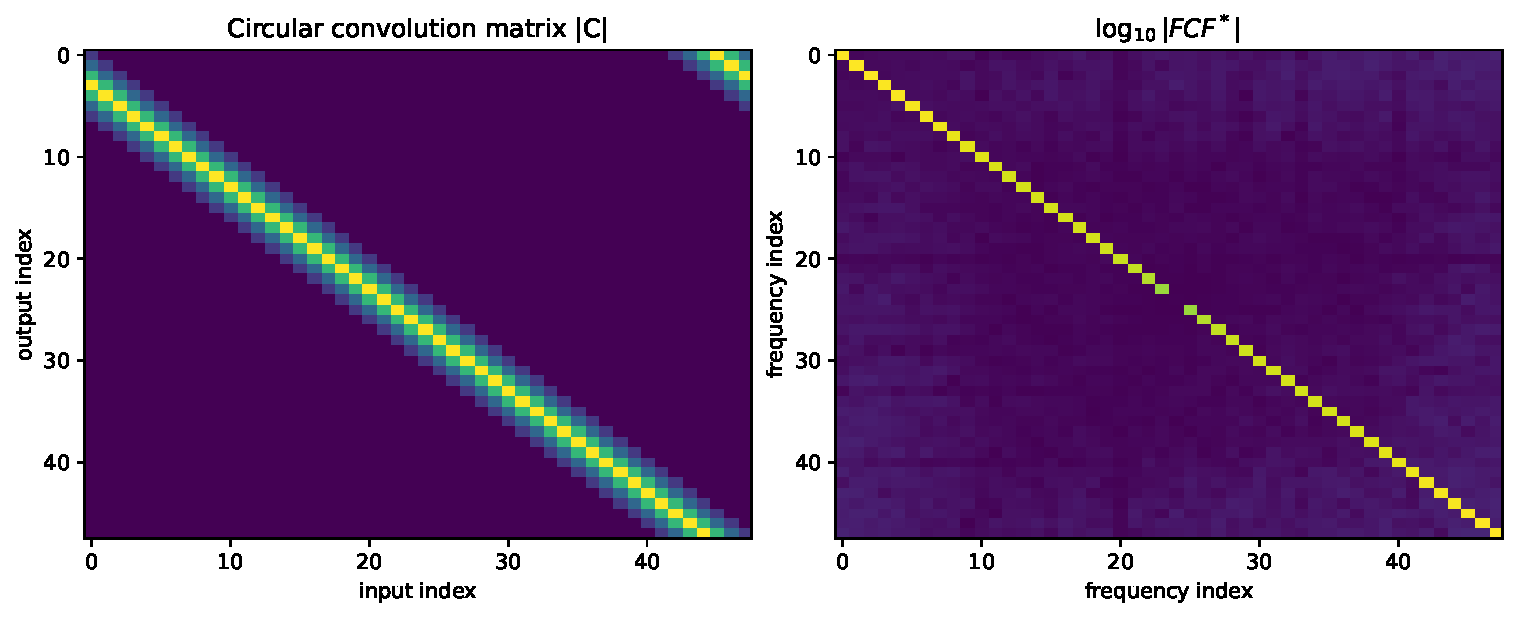
\includegraphics[width=0.92\textwidth]{dft_diagonalizes_circulant.pdf}
\caption{آزمایش عددی قطری‌شدن ماتریس کانولوشن دوری. نسبت نرم بخش خارج قطر به کل ماتریس در محاسبه
دوبل برابر \(\chthreeDftOffdiagRatio\) به دست آمد؛ مقدار غیرصفر باقیمانده صرفاً خطای گردکردن است.}
\label{fig:dft-diagonalization}
\end{figure}

\subsection{شرط‌های مرزی به‌عنوان بخشی از مدل}
چهار انتخاب رایج:
\begin{enumerate}
\item \textbf{صفر}: بیرون تصویر تاریک است؛ مناسب برخی مدل‌های پشتیبانی محدود، ولی ایجاد لبه مصنوعی می‌کند.
\item \textbf{دوری}: تصویر تکرار می‌شود؛ با \lr{DFT} سازگار، ولی در تصاویر طبیعی اغلب غیرواقعی است.
\item \textbf{انعکاسی}: مشتق نرمال روی مرز تقریباً صفر فرض می‌شود؛ معمولاً برای هموارسازی طبیعی‌تر است.
\item \textbf{تکرار آخرین مقدار}: ادامه ثابت؛ ساده ولی مشتق مرتبه بالاتر در مرز ناپیوسته است.
\end{enumerate}

\begin{figure}[H]
\centering
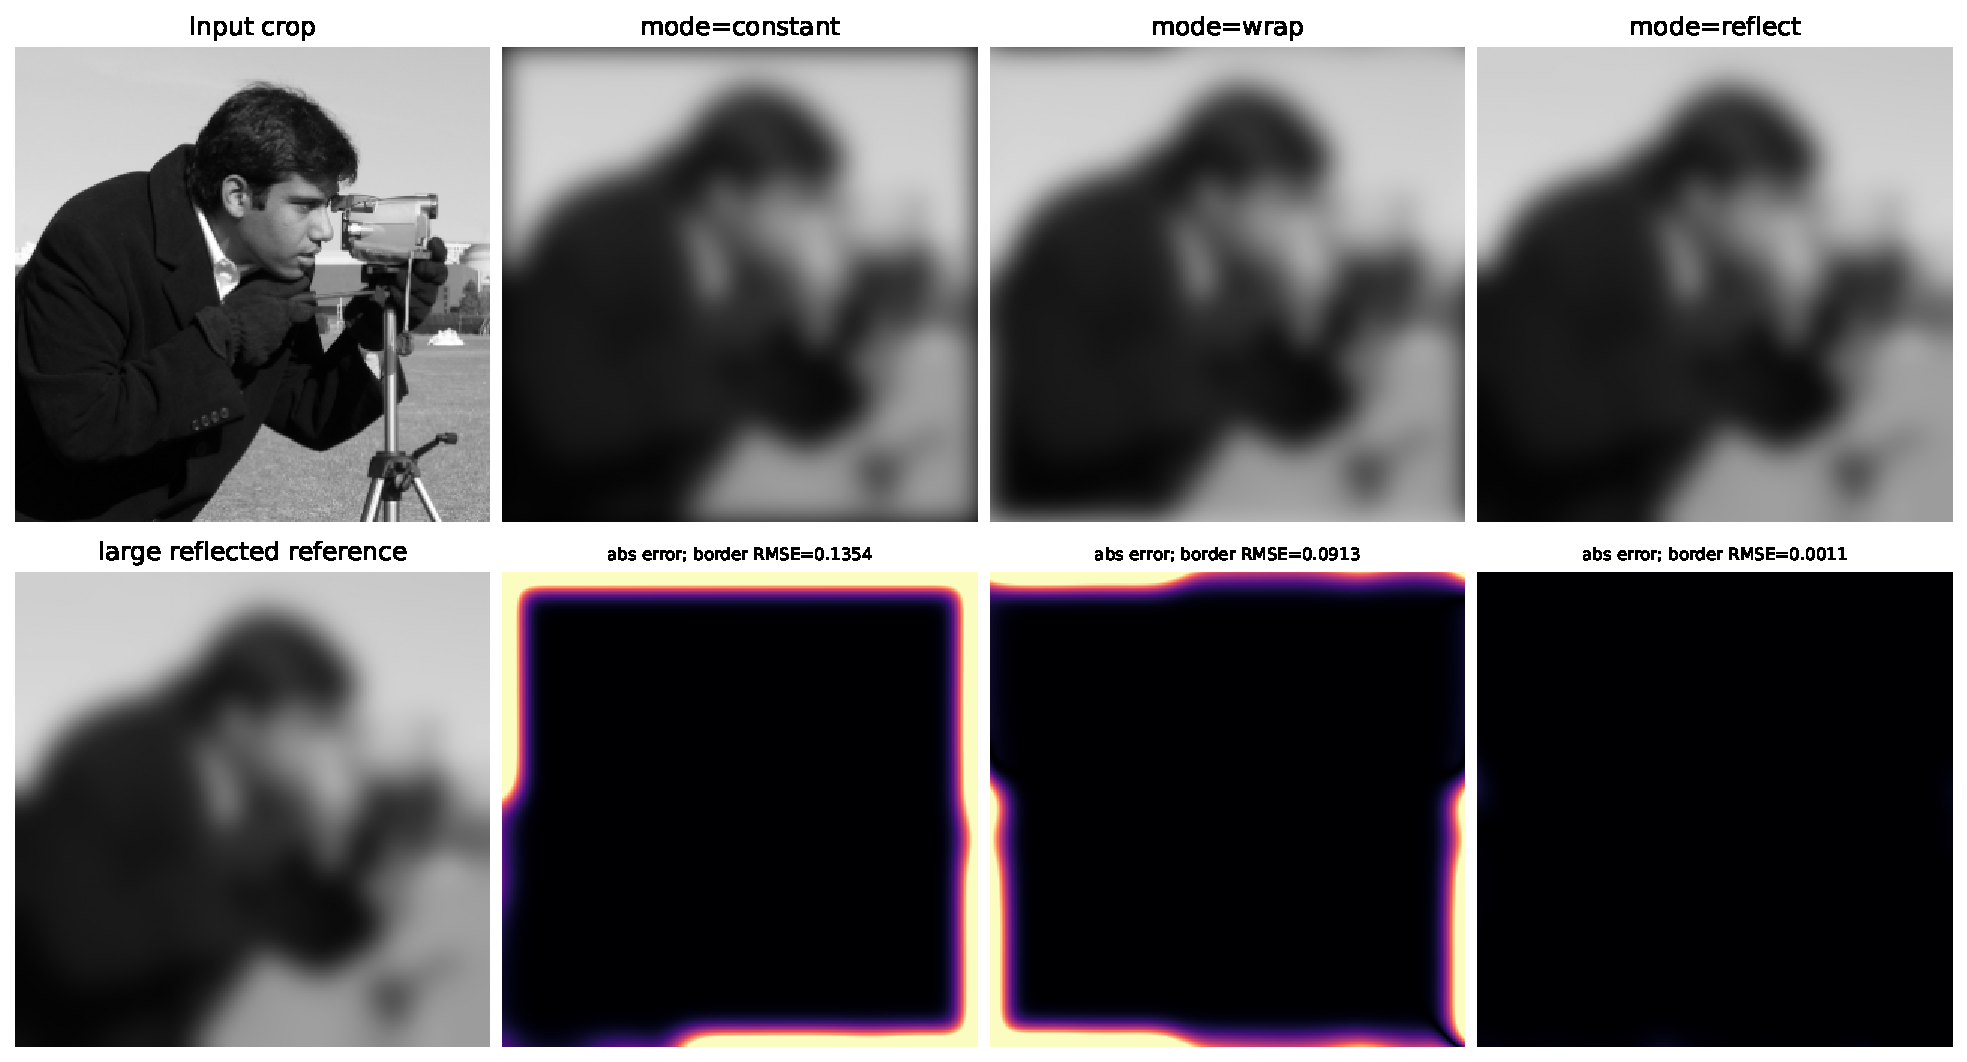
\includegraphics[width=0.96\textwidth]{boundary_conditions_real_image.pdf}
\caption{اثر واقعی شرط مرزی بر هموارسازی یک عکس. خطای \lr{RMSE} در نوار مرزی برای ادامه صفر، دوری و
انعکاسی به‌ترتیب \(\chthreeBoundaryConstantRmse\)، \(\chthreeBoundaryWrapRmse\) و
\(\chthreeBoundaryReflectRmse\) است. مقایسه با مرجع بزرگ انعکاسی انجام شده است.}
\label{fig:boundary}
\end{figure}

\begin{warningbox}
\lr{fftconvolve} معمولاً کانولوشن خطی با پد صفر را محاسبه می‌کند، نه کانولوشن انعکاسی. اگر خروجی آن با
\lr{GaussianBlur} دارای مرز انعکاسی مقایسه شود، اختلاف عمدتاً از الگوریتم نیست؛ از مدل مرز است.
\end{warningbox}

\section{عملگر الحاقی کانولوشن}

در مسائل معکوس و گرادیان‌گیری، الحاقی دقیق ضروری است. اگر
\begin{equation}
(Ax)[\vect n]=\sum_{\vect k}h[\vect k]x[\vect n-\vect k],
\end{equation}
با ضرب داخلی استاندارد و شرط مرزی سازگار، آنگاه
\begin{equation}
A^*z=\widetilde h*z,
\qquad
\widetilde h[\vect k]=\overline{h[-\vect k]}.
\label{eq:conv-adjoint}
\end{equation}
برای کرنل حقیقی و متقارن، \(A^*=A\). اما برای تاری حرکت جهت‌دار یا مشتق، این برابری برقرار نیست.

\begin{workshopbox}[آزمون الحاقی]
برای بردارهای تصادفی \(x,z\)، باید بررسی شود
\begin{equation}
\frac{|\inner{Ax}{z}-\inner{x}{A^*z}|}
{\max(1,|\inner{Ax}{z}|,|\inner{x}{A^*z}|)}<10^{-10}
\end{equation}
در محاسبه دوبل. این آزمون کوچک، خطاهای چرخاندن کرنل، برش خروجی و مرز را پیش از ورود به الگوریتم‌های
بازسازی آشکار می‌کند.
\end{workshopbox}

\section{تبدیل فوریه پیوسته}

برای \(f\in L^1(\R^d)\)، قرارداد این فصل چنین است:
\begin{equation}
\widehat f(\vect\omega)=\int_{\R^d}f(\vect r)e^{-i\vect\omega\cdot\vect r}\,d\vect r,
\label{eq:ctft}
\end{equation}
و اگر شرایط وارون‌سازی برقرار باشد،
\begin{equation}
f(\vect r)=\frac{1}{(2\pi)^d}\int_{\R^d}\widehat f(\vect\omega)
 e^{i\vect\omega\cdot\vect r}\,d\vect\omega.
\label{eq:ictft}
\end{equation}
قراردادهای دیگر ممکن است ضرایب \(2\pi\) را جابه‌جا کنند؛ فرمول‌ها باید با یک قرارداد واحد استفاده شوند.

\begin{theorem}[ریمان ـ لبگ]
اگر \(f\in L^1(\R^d)\)، آنگاه \(\widehat f\) پیوسته است و
\begin{equation}
\lim_{\norm{\vect\omega}\to\infty}\widehat f(\vect\omega)=0.
\end{equation}
\end{theorem}
این قضیه می‌گوید انتگرال‌پذیری مطلق موجب زوال طیف در فرکانس بالا می‌شود، اما نرخ زوال به همواری تابع وابسته است.

\begin{theorem}[پلانشرل و پارسوال]
تبدیل فوریه با نرمال‌سازی مناسب از \(L^1\cap L^2\) به یک عملگر واحدی روی \(L^2\) گسترش می‌یابد و
\begin{equation}
\norm{f}_2^2=\frac{1}{(2\pi)^d}\norm{\widehat f}_2^2,
\qquad
\inner{f}{g}=\frac{1}{(2\pi)^d}\inner{\widehat f}{\widehat g}.
\label{eq:parseval}
\end{equation}
\end{theorem}

\begin{proofbox}[چرا این قضیه برای تصویر حیاتی است؟]
رابطه \eqref{eq:parseval} اجازه می‌دهد انرژی خطا، نویز یا باقیمانده را در هر یک از دو حوزه محاسبه کنیم.
همچنین اگر فیلتر در حوزه فرکانس ضرب باشد، نرم عملگر روی \(L^2\) با بیشینه اندازه پاسخ فرکانسی کنترل می‌شود:
\begin{equation}
\norm{h*f}_2\le \esssup_{\omega}|H(\omega)|\,\norm f_2.
\end{equation}
\end{proofbox}

\subsection{قضیه کانولوشن}

\begin{theorem}[کانولوشن و ضرب]
اگر \(f,g\in L^1\)، آنگاه
\begin{equation}
\widehat{f*g}=\widehat f\,\widehat g.
\label{eq:conv-theorem}
\end{equation}
همچنین با قراردادهای مناسب،
\begin{equation}
\widehat{fg}=\frac{1}{(2\pi)^d}\widehat f*\widehat g.
\end{equation}
\end{theorem}

\begin{proof}
با استفاده از تونلی و تغییر متغیر \(\vect u=\vect r-\vect s\):
\begin{align}
\widehat{f*g}(\vect\omega)
&=\int\int f(\vect r-\vect s)g(\vect s)e^{-i\vect\omega\cdot\vect r}
 d\vect s d\vect r\\
&=\int g(\vect s)e^{-i\vect\omega\cdot\vect s}d\vect s
\int f(\vect u)e^{-i\vect\omega\cdot\vect u}d\vect u\\
&=\widehat f(\vect\omega)\widehat g(\vect\omega).
\end{align}
\end{proof}

\subsection{جدول خواص بنیادی}

\begin{longtable}{p{0.25\textwidth}p{0.31\textwidth}p{0.34\textwidth}}
\toprule
عمل در مکان & نتیجه در فرکانس & تفسیر تصویری\\
\midrule
\endfirsthead
\toprule
عمل در مکان & نتیجه در فرکانس & تفسیر تصویری\\
\midrule
\endhead
\(f(\vect r-\vect a)\) & \(e^{-i\omega\cdot a}\widehat f(\omega)\) & انتقال فقط فاز را تغییر می‌دهد.\\
\(e^{i\omega_0\cdot r}f(r)\) & \(\widehat f(\omega-\omega_0)\) & مدولاسیون طیف را جابه‌جا می‌کند.\\
\(f(A\vect r)\) & \(|\det A|^{-1}\widehat f(A^{-\mathsf T}\omega)\) & تغییر مقیاس/هندسه در دو حوزه معکوس است.\\
\(\partial^\alpha f\) & \((i\omega)^\alpha\widehat f\) & مشتق فرکانس بالا را تقویت می‌کند.\\
\(\vect r^\alpha f\) & \(i^{|\alpha|}\partial_\omega^\alpha\widehat f\) & تمرکز مکانی با همواری طیفی مرتبط است.\\
\(f*g\) & \(FG\) & سامانه LSI در هر فرکانس یک بهره مختلط دارد.\\
\(fg\) & \((2\pi)^{-d}F*G\) & برش و پنجره‌گذاری موجب پخش طیفی می‌شود.\\
\bottomrule
\end{longtable}

\section{سینوس‌ها تابع ویژه سامانه انتقال‌ناوردا هستند}

\begin{theorem}
برای سامانه کانولوشنی \(T_h f=h*f\)، نمایی مختلط \(e^{i\vect\omega_0\cdot\vect r}\) تابع ویژه است:
\begin{equation}
T_h e^{i\vect\omega_0\cdot\vect r}
=H(\vect\omega_0)e^{i\vect\omega_0\cdot\vect r}.
\label{eq:sin-eigen}
\end{equation}
\end{theorem}

\begin{proof}
\begin{align}
(h*e^{i\omega_0\cdot(\cdot)})(r)
&=\int h(s)e^{i\omega_0\cdot(r-s)}ds\\
&=e^{i\omega_0\cdot r}\int h(s)e^{-i\omega_0\cdot s}ds
=H(\omega_0)e^{i\omega_0\cdot r}.
\end{align}
\end{proof}

بنابراین سامانه فرکانس سینوس را عوض نمی‌کند؛ فقط دامنه و فاز آن را با مقدار ویژه \(H(\omega_0)\)
تغییر می‌دهد. این دقیقاً علت طبیعی‌بودن پایه فوریه برای تحلیل سامانه‌های انتقال‌ناوردا است.

\begin{figure}[H]
\centering
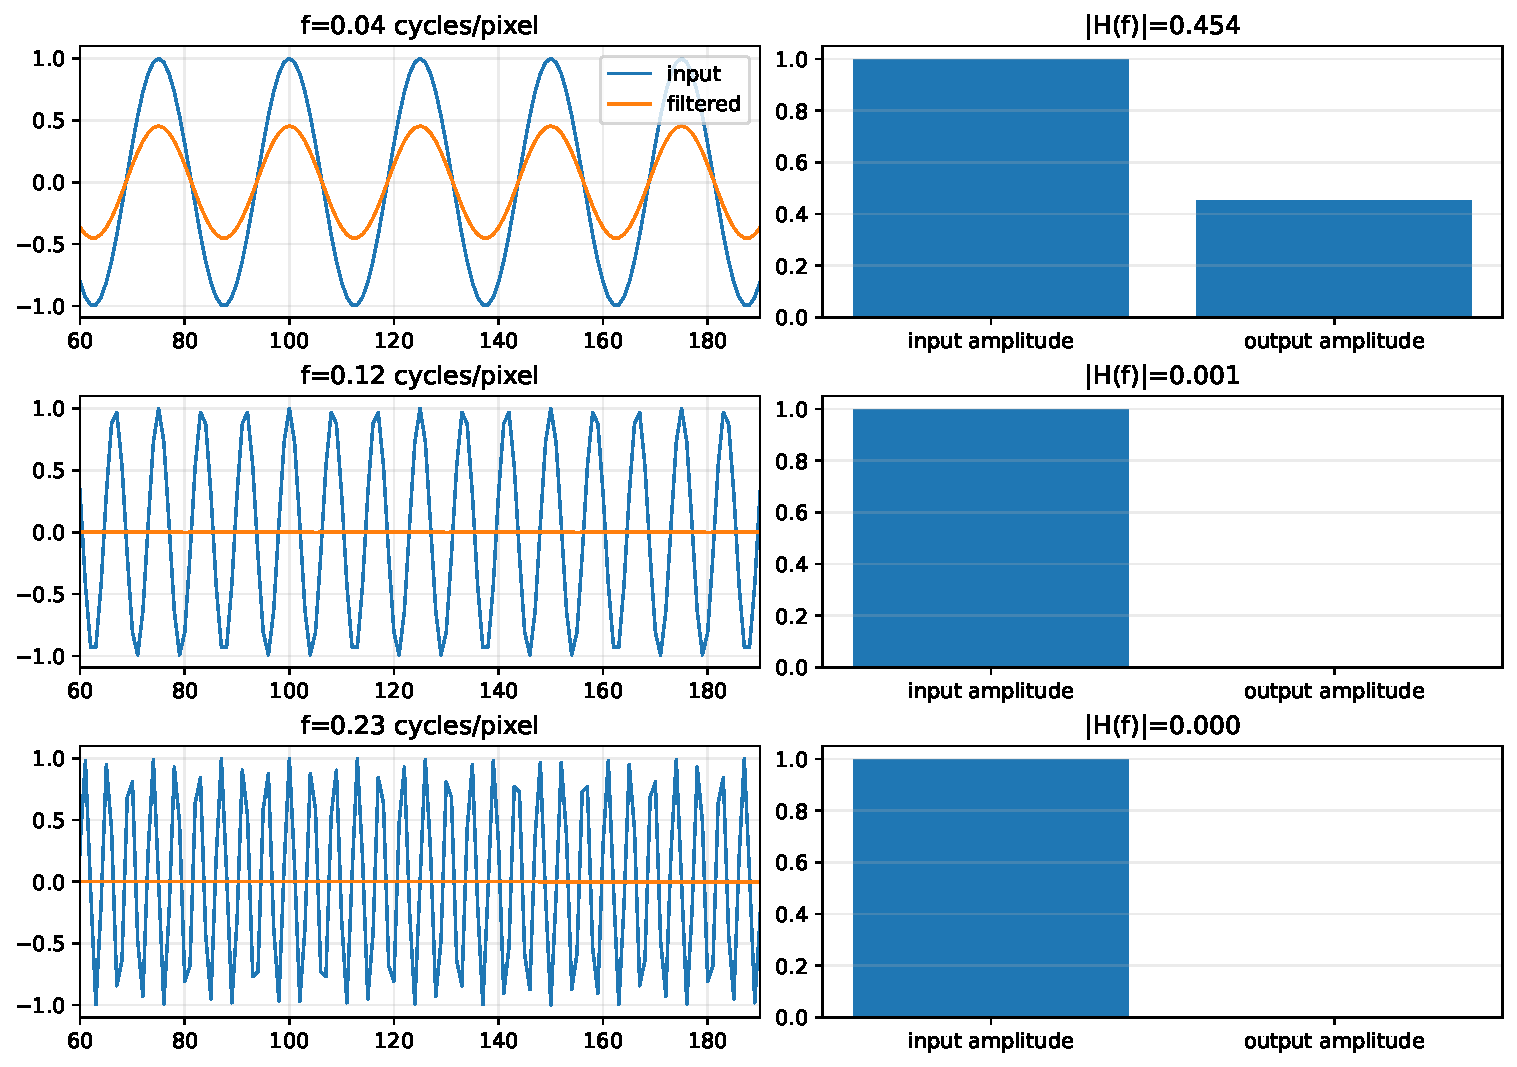
\includegraphics[width=0.9\textwidth]{lti_sinusoid_eigenfunctions.pdf}
\caption{سه سینوس با فرکانس متفاوت پس از فیلتر گاوسی. فرکانس حفظ می‌شود، اما بهره \(|H(f)|\) با افزایش
فرکانس کاهش می‌یابد. این آزمایش صورت عددی رابطه \eqref{eq:sin-eigen} است.}
\end{figure}

\section{دامنه و فاز: کدام‌یک ساختار را حمل می‌کند؟}

برای تصویر حقیقی، طیف مختلط را می‌نویسیم
\begin{equation}
F(\omega_x,\omega_y)=A(\omega_x,\omega_y)e^{i\phi(\omega_x,\omega_y)}.
\end{equation}
دامنه توزیع انرژی برحسب فرکانس و فاز هم‌ترازی مکانی مؤلفه‌ها را تعیین می‌کند. بدون فاز صحیح، لبه‌ها و
اجزای تصویر در مکان مناسب جمع نمی‌شوند.

\begin{figure}[H]
\centering
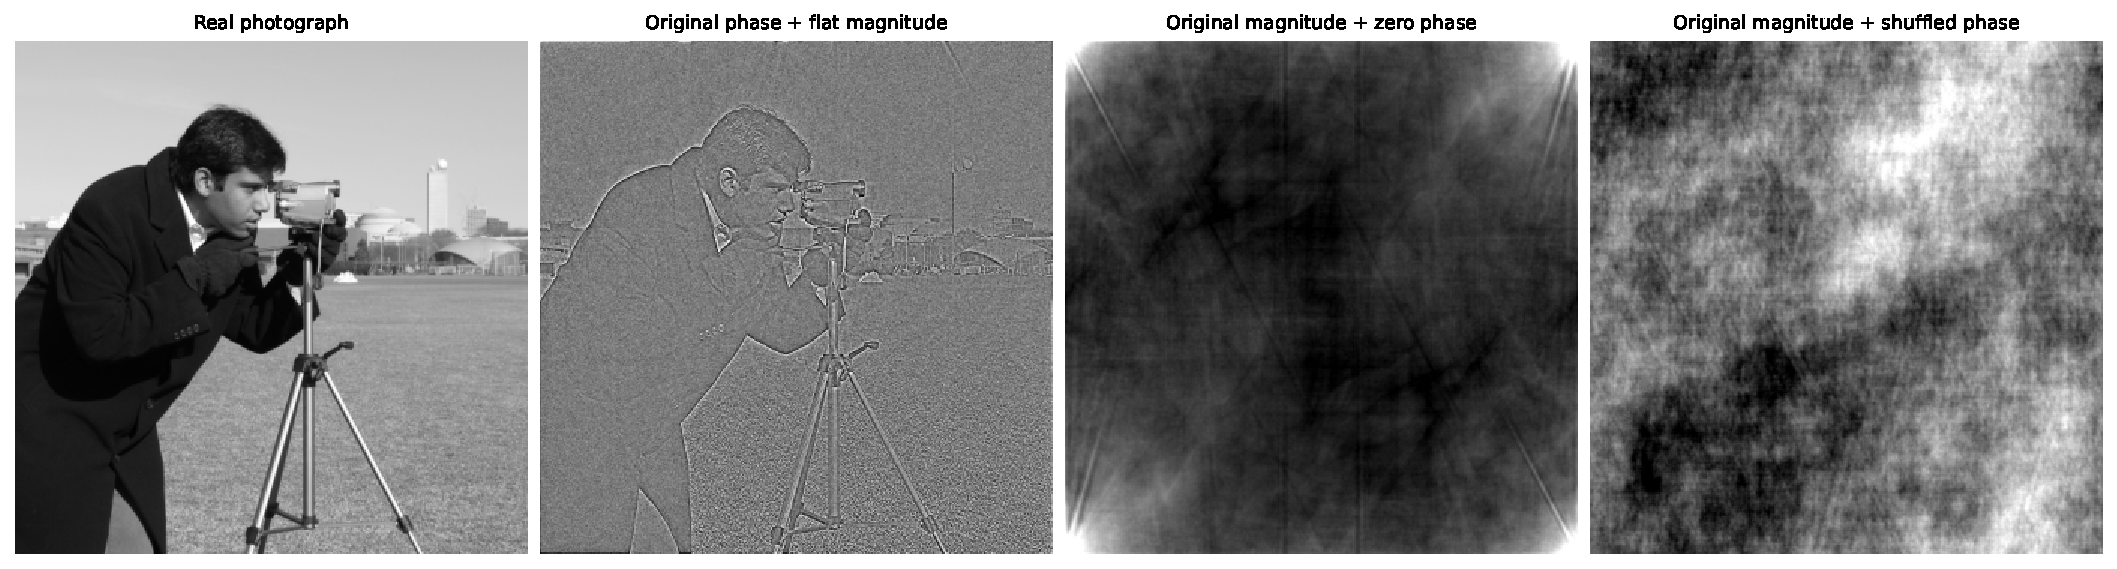
\includegraphics[width=0.98\textwidth]{phase_magnitude_real_image.pdf}
\caption{آزمایش روی یک عکس واقعی. بازسازی با فاز اصلی و دامنه تخت هنوز ساختار کلی را آشکار می‌کند؛ حفظ
دامنه و حذف/درهم‌ریزی فاز ساختار را از بین می‌برد. مقادیر \lr{SSIM} به‌ترتیب
\(\chthreePhaseOnlySsim\)، \(\chthreeMagnitudeOnlySsim\) و \(\chthreeShuffledPhaseSsim\) بوده‌اند.
این اعداد معیار کامل ادراک نیستند، اما نقش هم‌ترازی فازی را نشان می‌دهند.}
\label{fig:phase}
\end{figure}

\begin{warningbox}
جمله مشهور «فاز مهم‌تر از دامنه است» یک قضیه عمومی رتبه‌بندی نیست. اهمیت نسبی به تصویر، نرمال‌سازی و
وظیفه وابسته است. نتیجه دقیق‌تر این است: فاز اطلاعات مکان و هم‌ترازی مؤلفه‌های فوریه را حمل می‌کند و برای
بازسازی ساختارهای موضعی ضروری است؛ دامنه نیز انرژی، بافت و کنتراست طیفی را تعیین می‌کند.
\end{warningbox}

\section{تبدیل فوریه گسسته}

برای \(x[n]\)، \(n=0,\dots,N-1\)،
\begin{equation}
X[k]=\sum_{n=0}^{N-1}x[n]e^{-i2\pi kn/N},
\qquad k=0,\dots,N-1,
\label{eq:dft}
\end{equation}
و
\begin{equation}
x[n]=\frac{1}{N}\sum_{k=0}^{N-1}X[k]e^{i2\pi kn/N}.
\label{eq:idft}
\end{equation}

\subsection{ماتریس DFT و تعامد}
اگر \(W_N=e^{-i2\pi/N}\) و
\begin{equation}
(F_N)_{k,n}=\frac{1}{\sqrt N}W_N^{kn},
\end{equation}
آنگاه \(F_N\) واحدی است.

\begin{theorem}
\begin{equation}
F_N\herm F_N=I_N.
\end{equation}
\end{theorem}

\begin{proof}
درایه \((p,q)\) برابر
\begin{equation}
\frac{1}{N}\sum_{n=0}^{N-1}e^{i2\pi(p-q)n/N}
\end{equation}
است. اگر \(p=q\)، مجموع یک است؛ در غیر این صورت مجموع هندسی ریشه‌های واحد صفر می‌شود.
\end{proof}

\begin{corollary}[پارسوال گسسته]
با نرمال‌سازی واحدی،
\begin{equation}
\norm{F_Nx}_2=\norm{x}_2.
\end{equation}
در قرارداد رایج NumPy که تبدیل مستقیم بدون \(1/\sqrt N\) است،
\begin{equation}
\sum_n|x[n]|^2=\frac{1}{N}\sum_k|X[k]|^2.
\end{equation}
\end{corollary}

\subsection{DFT نمایش یک امتداد تناوبی است}
\lr{DFT} فرض نمی‌کند جهان فیزیکی تناوبی است، اما داده محدود را در پایه توابع تناوبی نمایش می‌دهد؛
بنابراین کانولوشن متناظر به‌طور طبیعی دوری است. برای به‌دست‌آوردن کانولوشن خطی طول \(N+M-1\)، باید
هر دو دنباله حداقل تا این طول پد شوند.

\begin{theorem}[قطری‌شدن کانولوشن دوری]
اگر \(C_h\) ماتریس دوری کانولوشن با \(h\) باشد،
\begin{equation}
C_h=F_N\herm\diag(\sqrt N F_Nh)F_N.
\label{eq:circulant-diag}
\end{equation}
در قرارداد DFT غیرواحدی، ضرایب مقیاس متناظر تغییر می‌کنند.
\end{theorem}

\begin{proof}
ستون‌های \(F_N\herm\) نمایی‌های مختلط گسسته‌اند. طبق خاصیت تابع ویژه، هر ستون با مقدار ویژه‌ای برابر
DFT کرنل مقیاس می‌شود. گردآوری این روابط برای همه ستون‌ها رابطه \eqref{eq:circulant-diag} را می‌دهد.
\end{proof}

\section{DFT دوبعدی و هندسه فرکانس}

برای تصویر \(M\times N\):
\begin{equation}
X[k,\ell]=\sum_{m=0}^{M-1}\sum_{n=0}^{N-1}
 x[m,n]e^{-i2\pi(km/M+\ell n/N)}.
\end{equation}
جدایی‌پذیری نمایی باعث می‌شود
\begin{equation}
X=F_M x F_N^{\mathsf T}
\end{equation}
و تبدیل با اعمال DFT روی سطرها و سپس ستون‌ها محاسبه شود.

\subsection{رابطه جهت در مکان و فرکانس}
یک نوار سینوسی با خطوط روشن موازی جهت \(\vect v\)، بردار فرکانس عمود بر آن خطوط دارد. لبه عمودی
انرژی را عمدتاً در امتداد محور افقی فرکانس پخش می‌کند، زیرا تغییر در راستای افقی رخ می‌دهد. این اصل پایه
طراحی فیلتر جهت‌دار و تفسیر طیف بافت است.

\subsection{تقارن هرمیتی}
اگر \(x[m,n]\in\R\)،
\begin{equation}
X[-k,-\ell]=\overline{X[k,\ell]}
\end{equation}
با اندیس‌های پیمانه‌ای. به همین دلیل \lr{rfft} تنها نیم‌صفحه مستقل را ذخیره می‌کند؛ اما نحوه چینش
فرکانس‌ها باید در ضرب کرنل و بازسازی رعایت شود.

\section{FFT: تغییر ریاضیات نیست، تغییر سازمان محاسبه است}

مقاله \lr{Cooley--Tukey} در سال ۱۹۶۵ الگوریتمی برای تجزیه محاسبه سری فوریه پیچیده ارائه کرد
\cite{cooley1965fft}. برای \(N=2^m\)، اندیس‌های زوج و فرد را جدا می‌کنیم:
\begin{align}
X[k]
&=\sum_{r=0}^{N/2-1}x[2r]W_N^{2rk}
+W_N^k\sum_{r=0}^{N/2-1}x[2r+1]W_N^{2rk}\\
&=E[k]+W_N^kO[k],
\end{align}
که \(E,O\) دو DFT طول \(N/2\) هستند. همچنین
\begin{equation}
X[k+N/2]=E[k]-W_N^kO[k].
\end{equation}
پس بازگشت
\begin{equation}
T(N)=2T(N/2)+O(N)
\end{equation}
دارد و
\begin{equation}
T(N)=O(N\log_2N).
\end{equation}

\begin{figure}[H]
\centering
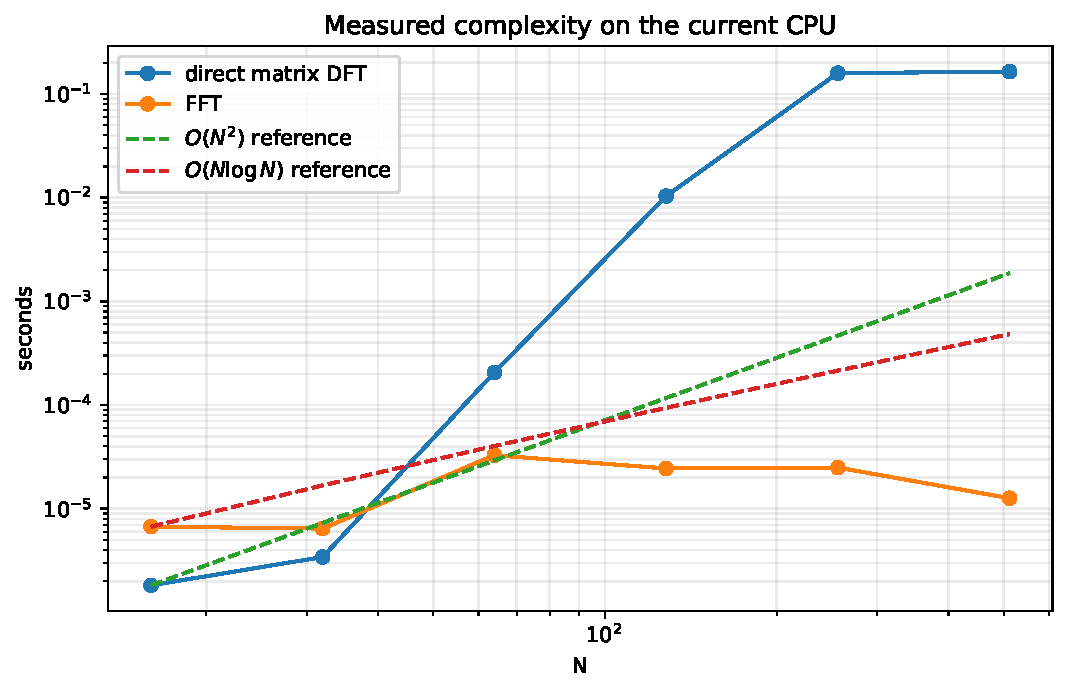
\includegraphics[width=0.76\textwidth]{fft_complexity_measured.pdf}
\caption{اندازه‌گیری زمان DFT ماتریسی و FFT روی همان پردازنده. در \(N=512\)، شتاب اندازه‌گیری‌شده
حدود \(\chthreeFftSpeedupNFiveOneTwo\) برابر بود. مقدار مطلق به سخت‌افزار و کتابخانه وابسته است؛ شیب
مقیاس‌پذیری مهم‌تر است.}
\end{figure}

\subsection{چه زمانی کانولوشن مستقیم سریع‌تر است؟}
برای تصویر \(MN\) و کرنل \(K\times K\):
\begin{equation}
C_{\rm direct}=O(MNK^2),
\qquad
C_{\rm FFT}=O(MN\log(MN))+O(MN).
\end{equation}
برای کرنل کوچک، سربار تبدیل، پد و حافظه باعث می‌شود روش مستقیم یا جدایی‌پذیر سریع‌تر باشد. برای کرنل
بزرگ، چند فیلتر با کرنل ثابت یا حل تکراری، FFT مزیت می‌یابد. در آزمایش فصل، کانولوشن FFT با کرنل
\(31\times31\) حدود \(\chthreeFftZeroSeconds\) ثانیه و کانولوشن مستقیم متقارن حدود
\(\chthreeSpatialSymmetricSeconds\) ثانیه طول کشید؛ مقایسه دقیق زمان باید با شرط مرزی یکسان انجام شود.

\section{نشت طیفی، پنجره و پد صفر}

اگر فقط قطعه‌ای محدود از تابع مشاهده شود، در واقع
\begin{equation}
x_{\rm obs}(t)=x(t)w(t)
\end{equation}
و بنابراین
\begin{equation}
X_{\rm obs}(\omega)=\frac{1}{2\pi}X*W.
\end{equation}
پنجره مستطیلی دارای تبدیل سینکی با لوب‌های جانبی آهسته‌کاه است، بنابراین انرژی یک مؤلفه غیرهم‌تراز با
شبکه DFT در چندین بین پخش می‌شود. پنجره‌های هان، همینگ و بلکمن لوب جانبی را کاهش می‌دهند، اما لوب اصلی
را پهن می‌کنند. این یک مصالحه میان تفکیک فرکانسی و نشت است.

\begin{keybox}[پد صفر چه می‌کند؟]
پد صفر نمونه‌های بیشتری از DTFT همان داده محدود فراهم می‌کند و نمودار طیف را نرم‌تر نشان می‌دهد، اما
اطلاعات یا تفکیک حقیقی جدید ایجاد نمی‌کند. تفکیک فیزیکی با طول مشاهده و پنجره تعیین می‌شود، نه صرفاً طول FFT.
\end{keybox}

\section{طراحی فیلتر در دو حوزه}

\subsection{حفظ مولفه DC}
برای فیلتر گسسته، پاسخ در فرکانس صفر
\begin{equation}
H(0,0)=\sum_{m,n}h[m,n].
\end{equation}
پس فیلتر هموارساز حفظ‌کننده میانگین باید مجموع یک داشته باشد؛ فیلتر مشتق یا بالاگذر حذف‌کننده ثابت باید
مجموع صفر داشته باشد.

\subsection{فیلتر جعبه‌ای}
کرنل یک‌بعدی طول \(K\):
\begin{equation}
h[n]=\frac{1}{K},\quad n=0,\dots,K-1
\end{equation}
پاسخ فرکانسی
\begin{equation}
H(e^{i\omega})=\frac{1}{K}e^{-i\omega(K-1)/2}
\frac{\sin(K\omega/2)}{\sin(\omega/2)}.
\end{equation}
صفرهای منظم و لوب‌های جانبی نشان می‌دهند که «میانگین‌گیری» یک پایین‌گذر یکنواخت نیست.

\subsection{گاوسی}
تبدیل فوریه گاوسی، گاوسی است:
\begin{equation}
g_\sigma(\vect r)=\frac{1}{2\pi\sigma^2}e^{-\norm r^2/(2\sigma^2)},
\qquad
G_\sigma(\vect\omega)=e^{-\sigma^2\norm\omega^2/2}.
\label{eq:gaussian-pair}
\end{equation}
گاوسی بدون نوسان و جدایی‌پذیر است و خاصیت نیم‌گروه دارد؛ این ویژگی‌ها آن را به هسته بنیادی فضای مقیاس
تبدیل می‌کنند.

\subsection{پایین‌گذر ایده‌آل و گیبس}
پاسخ ایده‌آل در یک بعد
\begin{equation}
H(\omega)=\mathbf 1_{[-\omega_c,\omega_c]}(\omega)
\end{equation}
کرنل سینکی با تکیه‌گاه نامتناهی می‌دهد. قطع ناگهانی در فرکانس موجب دنباله نوسانی در مکان و حلقه‌زنی کنار
لبه می‌شود.

\begin{figure}[H]
\centering
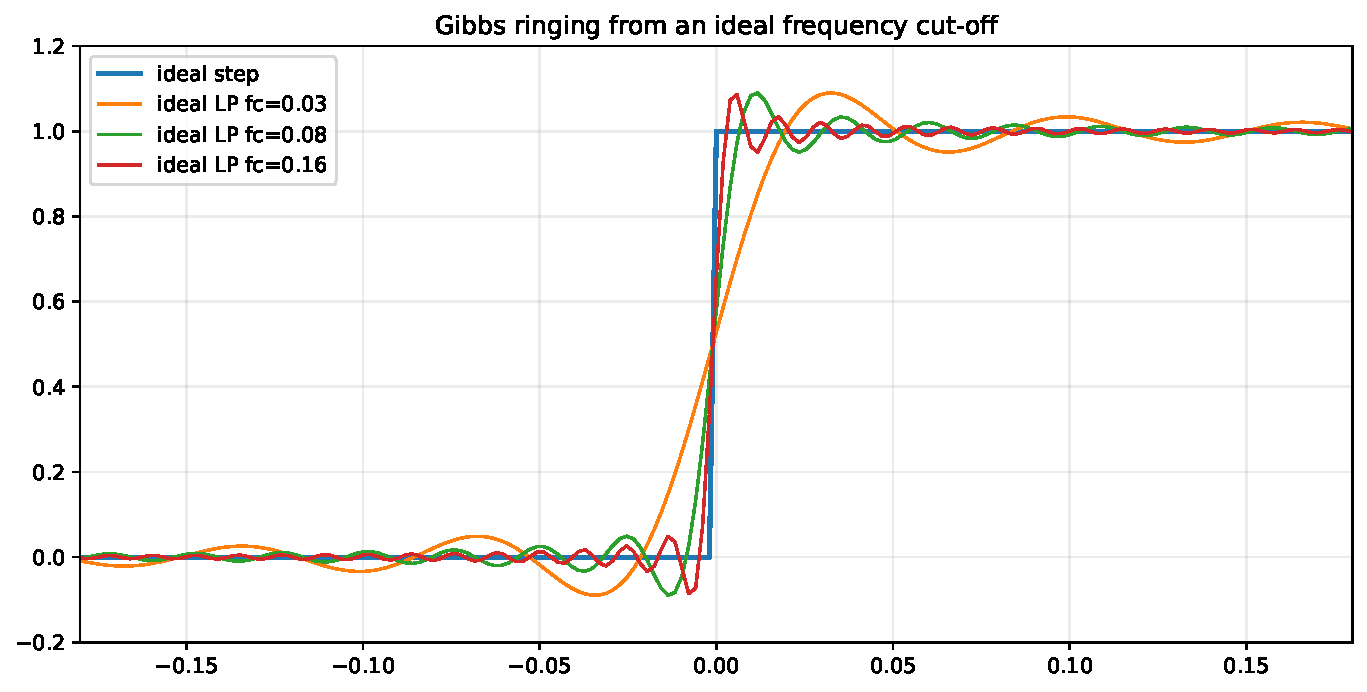
\includegraphics[width=0.76\textwidth]{gibbs_ringing.pdf}
\caption{پدیده گیبس در بازسازی پله با پایین‌گذر ایده‌آل. فراجهش با افزایش تعداد مؤلفه‌ها حذف نمی‌شود و
تقریباً نزدیک ۹ درصد باقی می‌ماند؛ فقط ناحیه نوسان باریک‌تر می‌شود.}
\end{figure}

\subsection{باتروورث و مصالحه گذار ـ حلقه‌زنی}
پایین‌گذر باتروورث دوبعدی:
\begin{equation}
H(\rho)=\frac{1}{1+(\rho/\rho_c)^{2n}}.
\end{equation}
افزایش مرتبه \(n\) گذار را تیزتر می‌کند، ولی پاسخ مکانی نوسانی‌تر می‌شود. هیچ طراحی بدون مصالحه میان
پهنای گذار، حلقه‌زنی، تکیه‌گاه و هزینه نیست.

\subsection{تیزکردن و ماسک غیرشارپ}
اگر \(L\) پایین‌گذر باشد، مؤلفه پرجزئیات \(x-Lx\) است و
\begin{equation}
y=x+\alpha(x-Lx).
\end{equation}
پاسخ فرکانسی
\begin{equation}
H_{\rm usm}(\omega)=1+\alpha(1-L(\omega))
\end{equation}
در فرکانس بالا بهره را افزایش می‌دهد. این عملیات «جزئیات» و نویز را از هم تشخیص نمی‌دهد.

\begin{figure}[H]
\centering
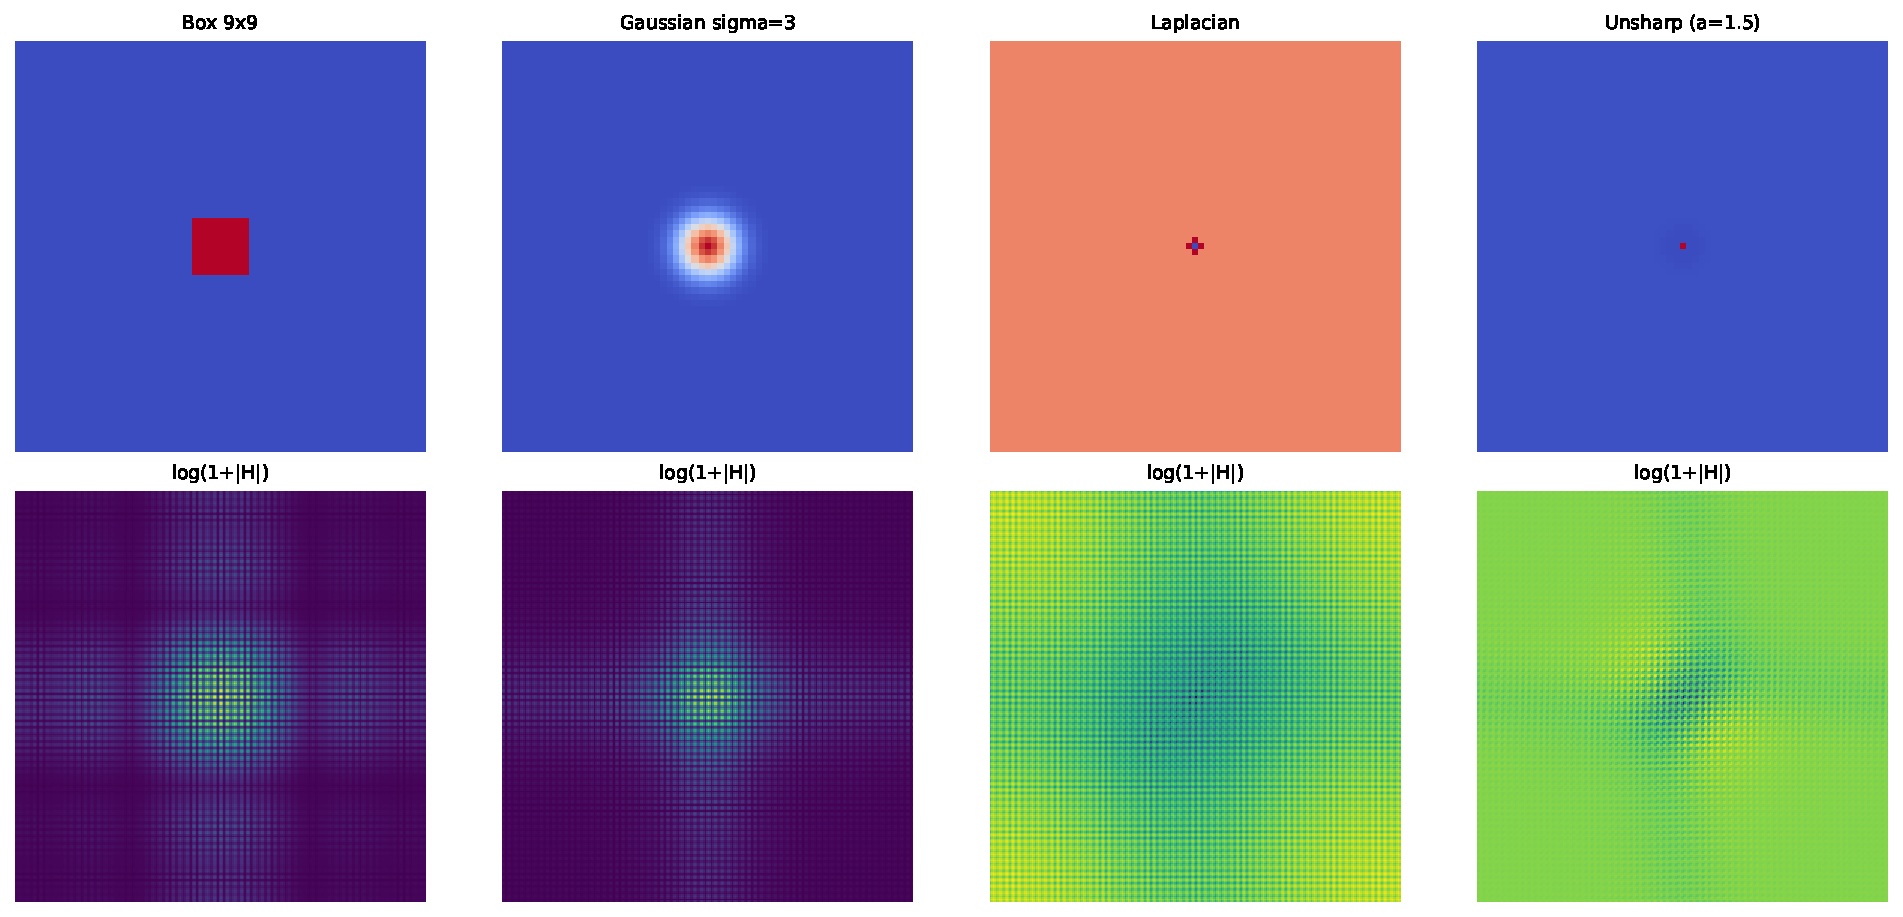
\includegraphics[width=0.97\textwidth]{spatial_frequency_filter_pairs.pdf}
\caption{جفت نمایش مکانی و فرکانسی چند فیلتر. هر طراحی باید هم شکل کرنل، هم اندازه پاسخ فرکانسی و در
صورت نیاز فاز را گزارش کند.}
\end{figure}

\section{مشتق، لاپلاسین و فرکانس بالا}

برای مشتق پیوسته:
\begin{equation}
\widehat{\frac{\partial f}{\partial x}}=i\omega_xF,
\qquad
\widehat{\nabla^2 f}=-(\omega_x^2+\omega_y^2)F.
\end{equation}
پس مشتق مؤلفه‌های پرفرکانس را تقویت می‌کند و نسبت به نویز حساس است. راه پایدارتر، مشتق‌گیری پس از
هموارسازی است:
\begin{equation}
\partial_x(g_\sigma*f)=(\partial_xg_\sigma)*f.
\end{equation}
این جابه‌جایی از خطی‌بودن و مشتق کانولوشن نتیجه می‌شود و پایه فیلترهای مشتق گاوسی است.

\begin{proposition}[تفاضل گاوسی تقریب لاپلاسین گاوسی]
برای \(k\) نزدیک یک،
\begin{equation}
g_{k\sigma}-g_\sigma
\approx (k-1)\sigma\frac{\partial g_\sigma}{\partial\sigma}
=(k-1)\sigma^2\nabla^2g_\sigma.
\end{equation}
\end{proposition}

\begin{proof}
بسط تیلور نسبت به \(\sigma\) می‌دهد
\begin{equation}
g_{k\sigma}=g_\sigma+(k-1)\sigma\partial_\sigma g_\sigma+O((k-1)^2).
\end{equation}
با مشتق مستقیم رابطه گاوسی یا معادله گرما، \(\sigma\partial_\sigma g_\sigma=\sigma^2\nabla^2g_\sigma\).
\end{proof}

\section{PSF، OTF و MTF}

در سامانه اپتیکی خطی انتقال‌ناوردا، پاسخ به نقطه \lr{PSF} است:
\begin{equation}
y=h_{\rm PSF}*x.
\end{equation}
تابع انتقال اپتیکی
\begin{equation}
\operatorname{OTF}(\vect f)=\FT\{h_{\rm PSF}\}(\vect f)
\end{equation}
و تابع انتقال مدولاسیون
\begin{equation}
\operatorname{MTF}(\vect f)=|\operatorname{OTF}(\vect f)|
\end{equation}
است. \lr{MTF} فاز را حذف می‌کند؛ بنابراین دو سامانه با MTF یکسان می‌توانند به دلیل فاز متفاوت تصویر
متفاوتی تولید کنند.

\subsection{ترکیب MTFها}
اگر زنجیره شامل اپتیک، حرکت، دهانه پیکسل و پردازش خطی باشد، تحت فرض LSI:
\begin{equation}
H_{\rm total}=H_{\rm optics}H_{\rm motion}H_{\rm pixel}H_{\rm processing}.
\end{equation}
پس MTF کل حاصل‌ضرب اندازه‌ها است. این رابطه فقط تا پیش از عملیات غیرخطی مانند کلیپ، دموزاییک تطبیقی یا
تیزکردن وابسته به محتوا معتبر است.

\subsection{روش لبه مایل}
استاندارد \lr{ISO 12233:2024} روش‌های اندازه‌گیری تفکیک و پاسخ فرکانس مکانی دوربین دیجیتال را مشخص
می‌کند \cite{iso12233_2024}. منطق لبه مایل چنین است:
\begin{enumerate}
\item تصویربرداری از یک لبه پُرکنتراست با زاویه اندک نسبت به شبکه پیکسل؛
\item برآورد مکان زیرپیکسلی لبه و تجمیع نمونه‌ها روی محور عمود بر لبه برای ساخت \lr{ESF} پُرنمونه؛
\item مشتق‌گیری از \lr{ESF} برای به‌دست‌آوردن \lr{LSF}؛
\item پنجره‌گذاری و تبدیل فوریه \lr{LSF}؛
\item نرمال‌سازی در فرکانس صفر و اعمال تصحیحات مشخص روش.
\end{enumerate}

\begin{figure}[H]
\centering
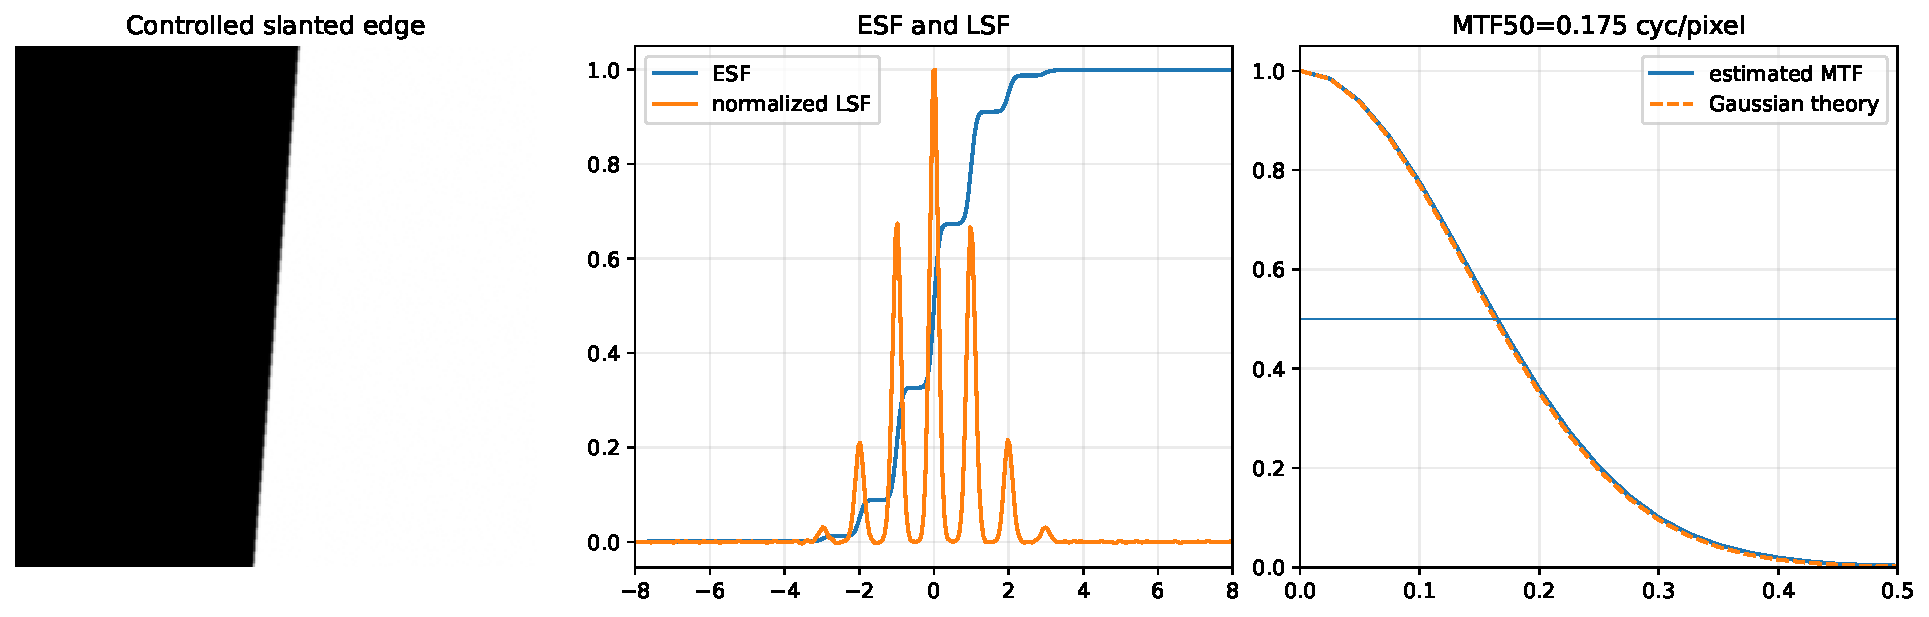
\includegraphics[width=0.95\textwidth]{slanted_edge_mtf.pdf}
\caption{پیاده‌سازی آموزشی منطق لبه مایل روی داده کنترل‌شده با تاری گاوسی. مقدار
\lr{MTF50} برآوردشده \(\chthreeSlantedEdgeMtfFiveZero\) چرخه بر پیکسل است. این شکل آزمون انطباق با
استاندارد نیست؛ اجرای استاندارد نیازمند هدف، نور، هندسه، پردازش و تصحیحات تعریف‌شده در سند است.}
\end{figure}

\begin{warningbox}
گزارش «رزولوشن دوربین» بدون تعیین خروجی RAW یا JPEG، جهت اندازه‌گیری، شارپ‌سازی، کنتراست هدف، میدان
تصویر و واحد فرکانس ناقص است. MTF ویژگی کل زنجیره است، نه فقط تعداد مگاپیکسل.
\end{warningbox}

\section{فیلتر معکوس و صفرهای پاسخ فرکانسی}

اگر
\begin{equation}
Y(\omega)=H(\omega)X(\omega)+N(\omega),
\end{equation}
فیلتر معکوس صوری
\begin{equation}
\widehat X_{\rm inv}=\frac{Y}{H}=X+\frac{N}{H}
\end{equation}
است. هرجا \(|H|\) کوچک باشد، نویز شدیداً تقویت می‌شود؛ اگر \(H=0\)، مؤلفه متناظر از داده قابل بازیابی
نیست. این همان بدوضعی فصل اول در پایه‌ای است که عملگر را قطری می‌کند.

\begin{keybox}[رابطه با مقادیر منفرد]
برای کانولوشن دوری، اندازه مقادیر DFT کرنل همان مقادیر منفرد تا ترتیب و فاز مناسب است. بنابراین
\begin{equation}
\cond(C_h)\approx\frac{\max_k|H[k]|}{\min_k|H[k]|}
\end{equation}
اگر مخرج غیرصفر باشد. افت MTF در فرکانس بالا به زبان عددی یعنی کاهش مقدار منفرد و افزایش حساسیت وارون‌سازی.
\end{keybox}

فصل پنجم وینر، تیکانوف، TV و روش‌های پروگزیمال را کامل بررسی می‌کند. در اینجا نکته بنیادی این است که
تحلیل فرکانسی محل از دست‌رفتن اطلاعات و تقویت نویز را آشکار می‌کند، اما خودِ آن جایگزین پیشین و منظم‌سازی نیست.

\section{فضای مقیاس گاوسی}

ساختارهای تصویری در یک مقیاس ثابت وجود ندارند. یک خراش، سلول، ساختمان یا ابر در بازه‌های متفاوتی از
تفکیک ظاهر می‌شود. نمایش فضای مقیاس خطی را تعریف می‌کنیم:
\begin{equation}
L(\vect r;t)=g(\vect r;t)*f(\vect r),
\qquad
g(\vect r;t)=\frac{1}{(4\pi t)^{d/2}}e^{-\norm r^2/(4t)},
\label{eq:scale-space}
\end{equation}
که \(t=\sigma^2/2\) در این قرارداد است.

\subsection{اصول ساختاری}
صورت‌های دقیق قضیه یکتایی بسته به فرض‌ها متفاوت‌اند، اما هسته عمومی نظریه \lr{Koenderink} و
\lr{Lindeberg} چنین است \cite{koenderink1984structure,lindeberg1994scale}:
\begin{itemize}
\item خطی‌بودن؛
\item انتقال‌ناوردایی؛
\item همسانگردی فضایی؛
\item خاصیت نیم‌گروه در مقیاس؛
\item پیوستگی در مقیاس؛
\item عدم ایجاد ساختار موضعی جدید یا اصل عدم تقویت اکسترمم‌ها.
\end{itemize}
تحت این اصول، خانواده هسته‌ها گاوسی است.

\begin{theorem}[خاصیت نیم‌گروه گاوسی]
\begin{equation}
g(\cdot;t_1)*g(\cdot;t_2)=g(\cdot;t_1+t_2).
\label{eq:gaussian-semigroup}
\end{equation}
در پارامتر \(\sigma\):
\begin{equation}
g_{\sigma_1}*g_{\sigma_2}=g_{\sqrt{\sigma_1^2+\sigma_2^2}}.
\end{equation}
\end{theorem}

\begin{proof}
با رابطه \eqref{eq:gaussian-pair}، تبدیل فوریه طرف چپ
\begin{equation}
e^{-t_1\norm\omega^2}e^{-t_2\norm\omega^2}
=e^{-(t_1+t_2)\norm\omega^2}
\end{equation}
است که تبدیل گاوسی با پارامتر \(t_1+t_2\) است. یکتایی تبدیل فوریه نتیجه را می‌دهد.
\end{proof}

\begin{figure}[H]
\centering
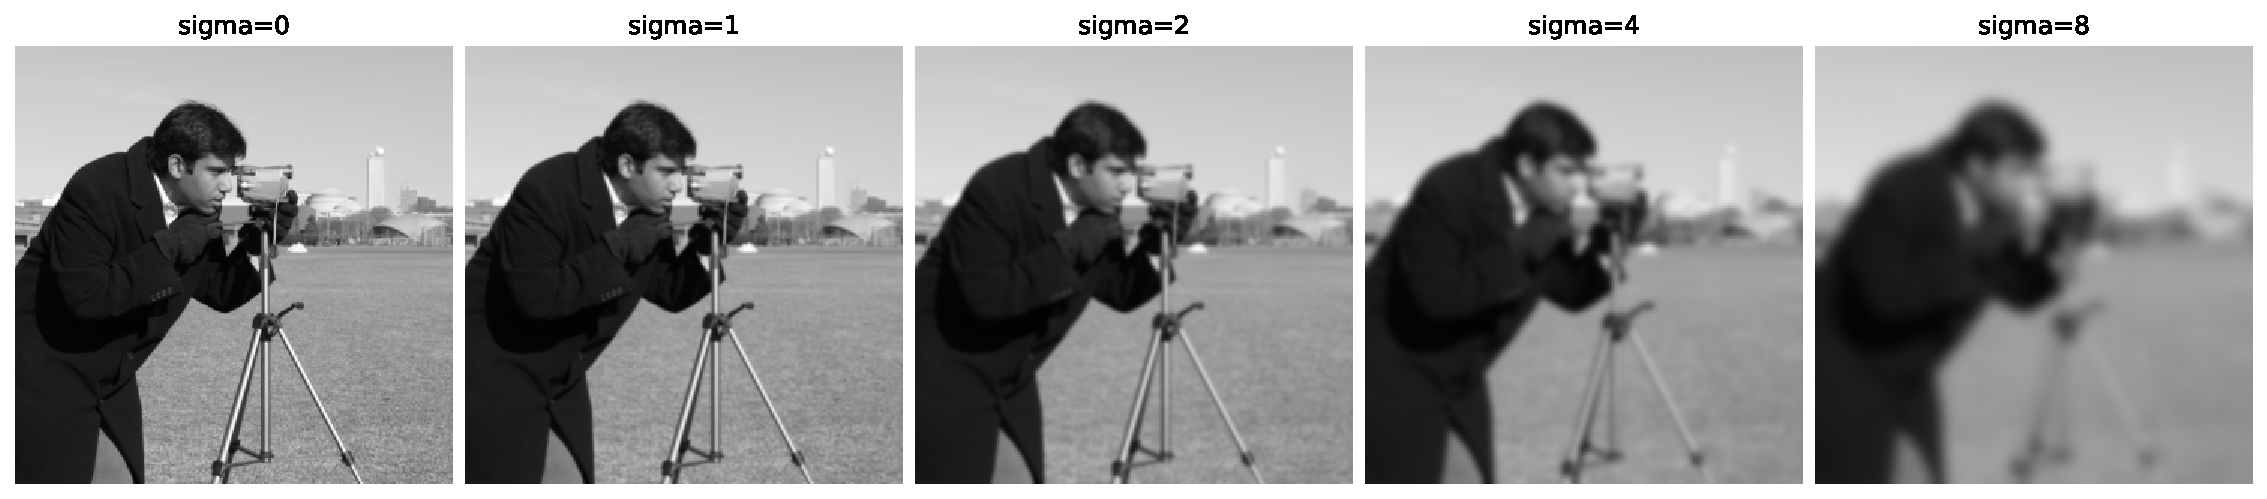
\includegraphics[width=0.98\textwidth]{gaussian_scale_space_real.pdf}
\caption{فضای مقیاس گاوسی یک عکس واقعی. با افزایش \(\sigma\)، جزئیات کوچک حذف می‌شوند ولی ساختارهای
درشت باقی می‌مانند. خطای نسبی آزمون نیم‌گروه عددی برابر \(\chthreeSemigroupRelativeError\) بود.}
\end{figure}

\subsection{رابطه با معادله گرما}

\begin{theorem}
تابع \(L(\vect r;t)=g_t*f\) حل معادله گرما است:
\begin{equation}
\frac{\partial L}{\partial t}=\nabla^2L,
\qquad
L(\vect r;0)=f(\vect r)
\label{eq:heat}
\end{equation}
در قرارداد هسته \eqref{eq:scale-space}.
\end{theorem}

\begin{proof}
در حوزه فرکانس،
\begin{equation}
\widehat L(\omega;t)=e^{-t\norm\omega^2}\widehat f(\omega).
\end{equation}
پس
\begin{equation}
\partial_t\widehat L=-\norm\omega^2\widehat L
=\widehat{\nabla^2L}.
\end{equation}
وارون‌سازی فوریه رابطه را می‌دهد.
\end{proof}

\subsection{اصل بیشینه و عدم ایجاد اکسترمم}
معادله گرما دارای اصل بیشینه است: درون دامنه، بیشینه جدید بالاتر از بیشینه اولیه ایجاد نمی‌شود. در یک بعد،
تعداد عبورهای صفر و اکسترمم‌ها با مقیاس افزایش نمی‌یابد، هرچند در پیاده‌سازی گسسته شمارش می‌تواند به
نحوه نمونه‌برداری و مرز حساس باشد.

\begin{figure}[H]
\centering
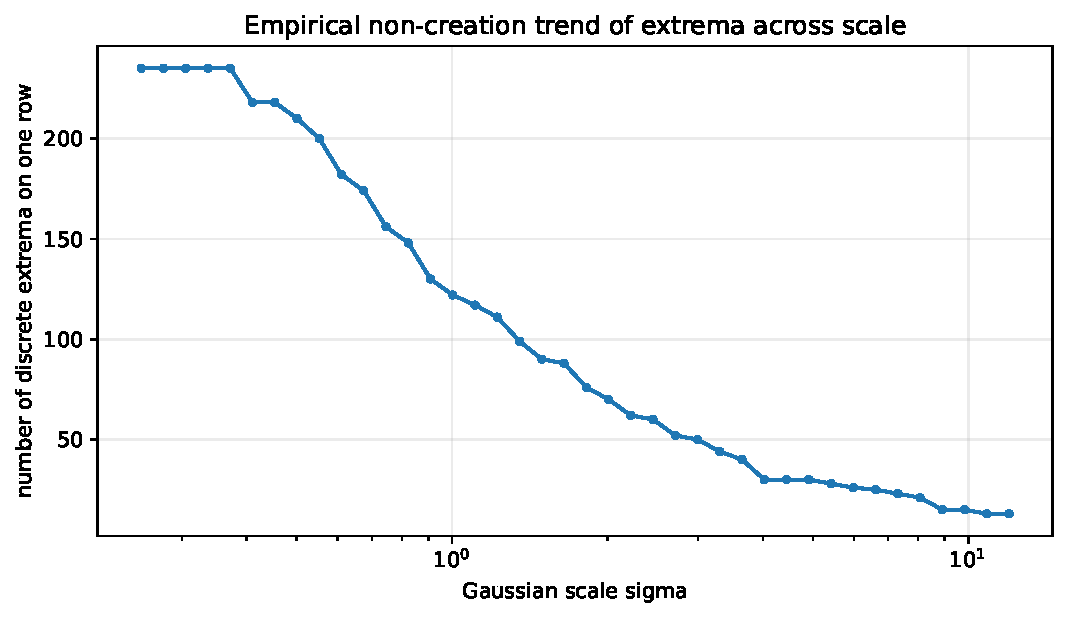
\includegraphics[width=0.7\textwidth]{scale_space_extrema.pdf}
\caption{شمارش تجربی اکسترمم‌های یک سطر عکس در مقیاس‌های گاوسی. شمارش از \(\chthreeExtremaInitial\)
به \(\chthreeExtremaFinal\) کاهش یافته است. این آزمایش شهود اصل عدم ایجاد ساختار را نشان می‌دهد، نه
اثبات گسسته برای هر الگوریتم.}
\end{figure}

\subsection{مشتق نرمال‌شده نسبت به مقیاس}
دامنه مشتق با افزایش \(\sigma\) کاهش می‌یابد. برای مقایسه پاسخ‌ها در مقیاس‌های متفاوت، مشتق نرمال‌شده
\begin{equation}
\partial_{\xi_i}=t^{\gamma/2}\partial_{x_i}
\end{equation}
به کار می‌رود. انتخاب \(\gamma=1\) در بسیاری از مسائل انتخاب خودکار مقیاس، هم‌وردایی مناسب نسبت به تغییر
اندازه می‌دهد \cite{lindeberg1998automatic}.

\section{هرم گاوسی و لاپلاسی}

\subsection{هرم گاوسی}
\begin{equation}
G_{j+1}=\downarrow_2(h*G_j),
\qquad G_0=f.
\end{equation}
هموارسازی پیش از کاهش نرخ ضروری است. اگر هر بعد نصف شود، تعداد کل نمونه‌ها در هرم نامتناهی دوبعدی
\begin{equation}
MN\left(1+\frac14+\frac1{16}+\cdots\right)=\frac43MN
\end{equation}
است.

\subsection{هرم لاپلاسی}
هرم لاپلاسی \lr{Burt--Adelson} اختلاف میان سطح و پیش‌بینی بازگسترش‌یافته سطح بعد است
\cite{burt1983laplacian}:
\begin{equation}
L_j=G_j-\operatorname{expand}(G_{j+1}),
\qquad L_J=G_J.
\end{equation}
بازسازی:
\begin{equation}
G_j=L_j+\operatorname{expand}(G_{j+1}).
\end{equation}
در صورتی که همان عملگر گسترش استفاده شود، بازسازی جبری کامل است؛ کیفیت فشرده‌سازی پس از کوانتیزه‌کردن
ضرایب مسئله دیگری است.

\begin{figure}[H]
\centering
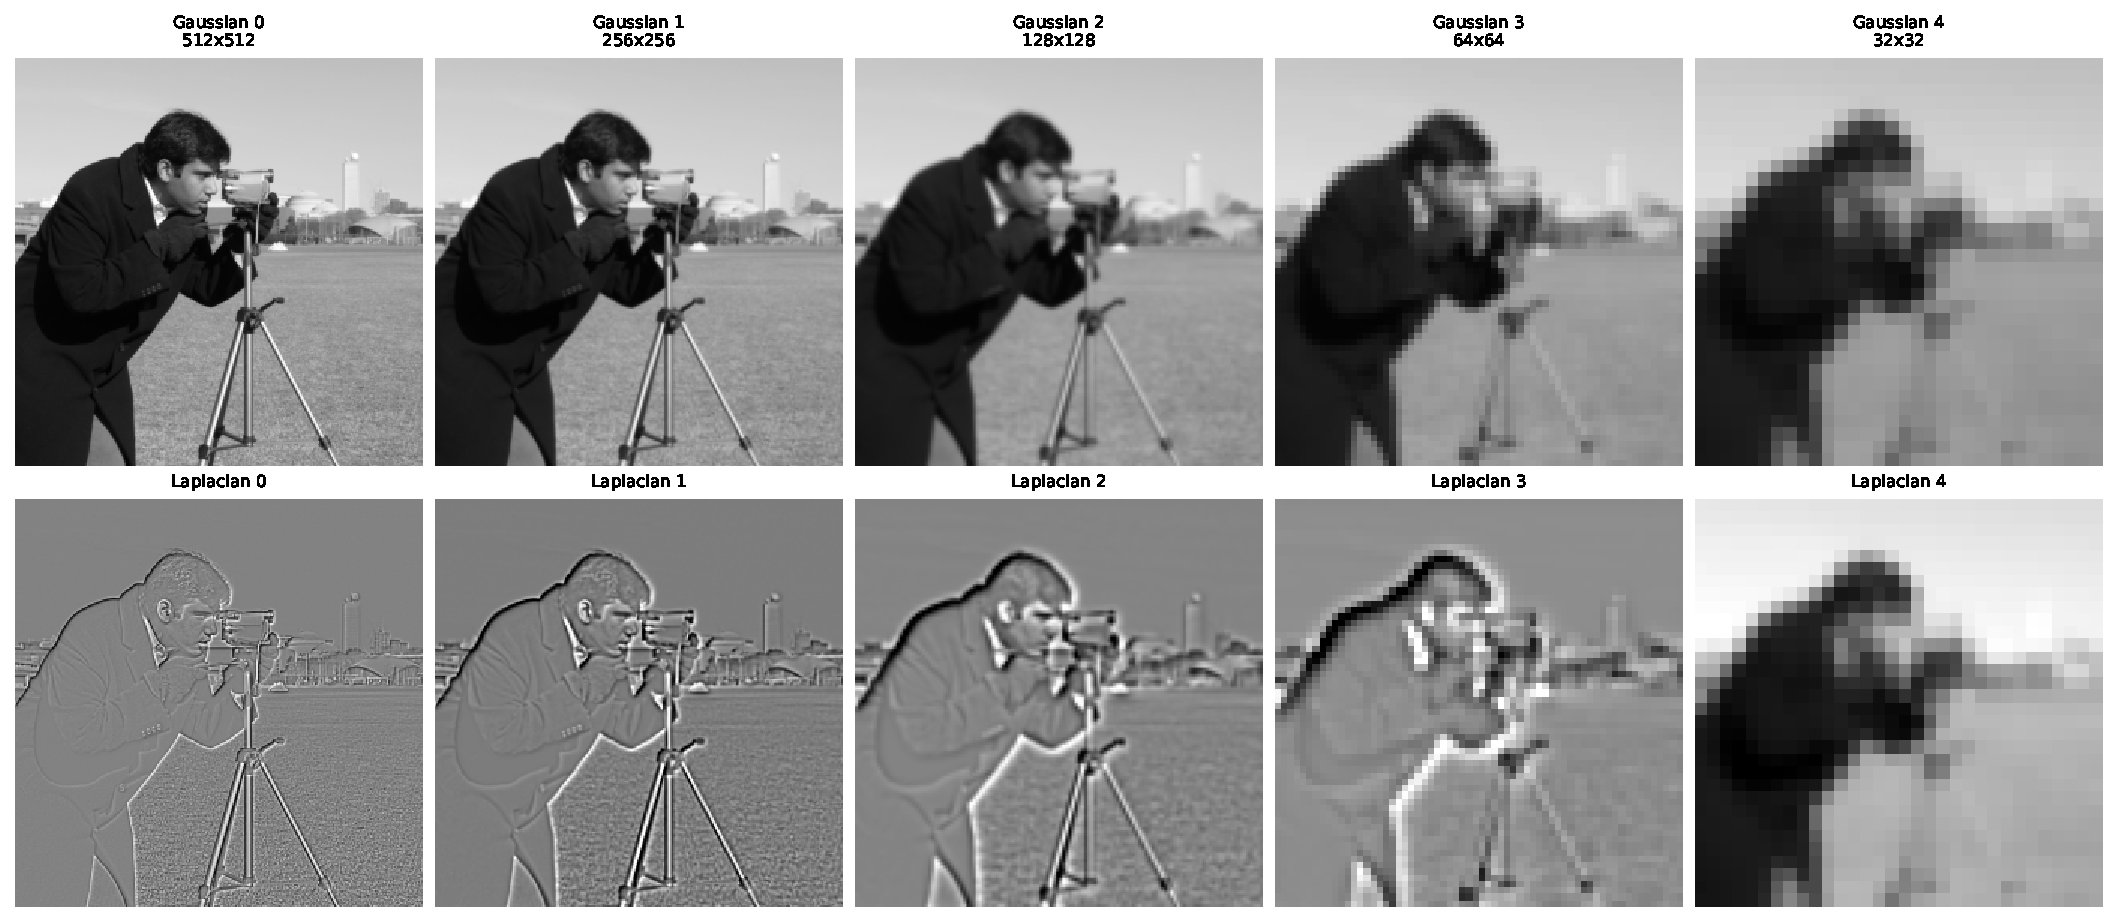
\includegraphics[width=0.98\textwidth]{gaussian_laplacian_pyramids.pdf}
\caption{هرم گاوسی و لاپلاسی یک عکس واقعی. بیشینه خطای بازسازی در محاسبه دوبل
\(\chthreeLaplacianReconstructionMaxAbs\) و خطای نسبی \(\chthreeLaplacianReconstructionRelLTwo\)
بود؛ این آزمون باید در هر پیاده‌سازی هرم وجود داشته باشد.}
\end{figure}

\section{تحلیل مکان ـ فرکانس و اصل عدم قطعیت}

فوریه مکان را حذف می‌کند: می‌دانیم چه فرکانسی وجود دارد، نه کجا. برای رویدادهای موضعی، تابع پنجره‌ای لازم است.

\begin{theorem}[اصل عدم قطعیت هایزنبرگ ـ گابور]
اگر \(f\in L^2(\R)\)، \(tf(t)\in L^2\)، \(f'\in L^2\)، و میانگین‌های مکان و فرکانس صفر شده باشند،
آنگاه با قرارداد فرکانس زاویه‌ای
\begin{equation}
\left(\int t^2|f(t)|^2dt\right)
\left(\frac{1}{2\pi}\int \omega^2|\widehat f(\omega)|^2d\omega\right)
\ge \frac14\norm f_2^4.
\label{eq:uncertainty}
\end{equation}
برابری برای گاوسی رخ می‌دهد.
\end{theorem}

\begin{proof}[طرح اثبات]
با انتگرال‌گیری جزءبه‌جز و فرض زوال مرزی،
\begin{equation}
\norm f_2^2=-2\Re\int t f'(t)\overline{f(t)}dt.
\end{equation}
نامساوی کوشی ـ شوارتس می‌دهد
\begin{equation}
\norm f_2^4\le4\norm{tf}_2^2\norm{f'}_2^2.
\end{equation}
با پلانشرل، \(\norm{f'}_2^2=(2\pi)^{-1}\int\omega^2|\widehat f|^2d\omega\). شرط برابری کوشی
معادله \(f'=-ctf\) است که حل گاوسی دارد.
\end{proof}

\subsection{تبدیل فوریه کوتاه‌زمان/مکان}
برای پنجره \(g\):
\begin{equation}
V_gf(\tau,\omega)=\int f(t)\overline{g(t-\tau)}e^{-i\omega t}dt.
\end{equation}
تفکیک مکان و فرکانس با پهنای پنجره ثابت کنترل می‌شود: پنجره باریک مکان خوب و فرکانس ضعیف، پنجره پهن
برعکس. مقاله کلاسیک گابور این سلول‌های زمان ـ فرکانس را در زبان نظریه ارتباط صورت‌بندی کرد
\cite{gabor1946communication}.

\section{فیلترهای گابور و جهت}

اتم گابور دوبعدی:
\begin{equation}
g_{\theta,\omega_0}(\vect r)
=\exp\left(-\frac{x_\theta^2}{2\sigma_x^2}-\frac{y_\theta^2}{2\sigma_y^2}\right)
 e^{i\omega_0x_\theta},
\end{equation}
که
\begin{equation}
\begin{bmatrix}x_\theta\\y_\theta\end{bmatrix}
=\begin{bmatrix}\cos\theta&\sin\theta\\-\sin\theta&\cos\theta\end{bmatrix}
\begin{bmatrix}x\\y\end{bmatrix}.
\end{equation}
گاوسی مکان را محدود و حامل سینوسی فرکانس و جهت را انتخاب می‌کند. بخش حقیقی زوج و بخش موهومی فرد است؛
اندازه پاسخ مختلط نسبت به فاز موضعی مقاوم‌تر است.

\begin{figure}[H]
\centering
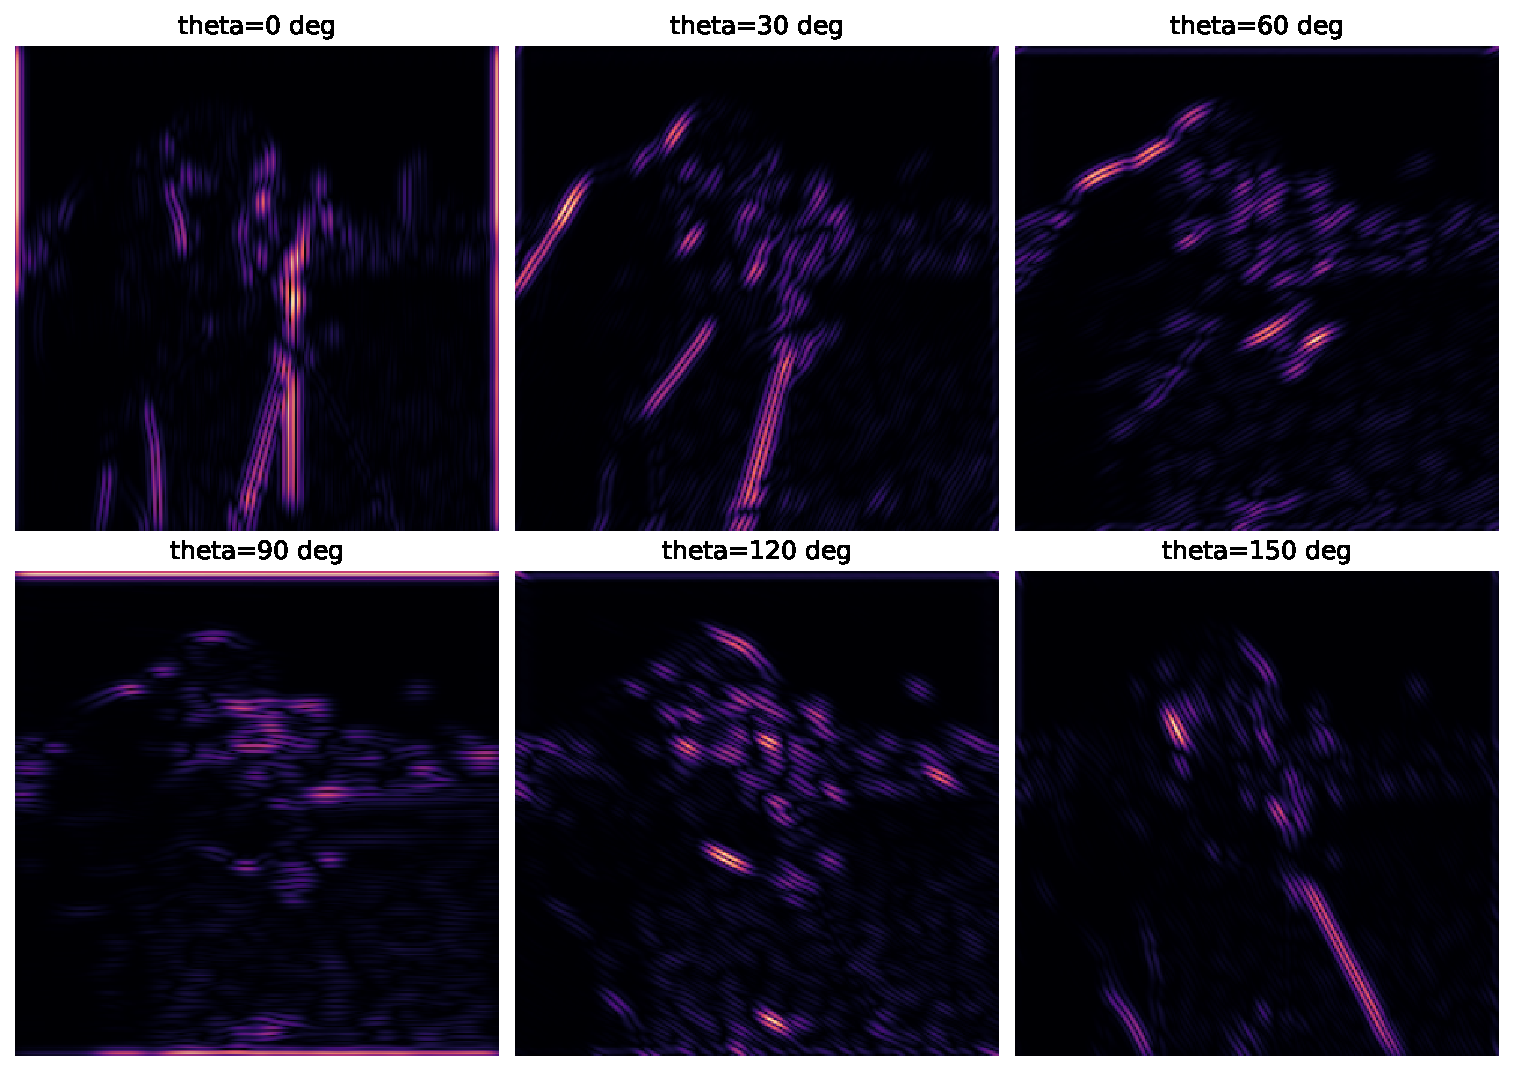
\includegraphics[width=0.88\textwidth]{gabor_orientation_bank.pdf}
\caption{اندازه پاسخ بانک گابور در شش جهت روی عکس واقعی. بافت و لبه‌هایی که عمود بر بردار فرکانس فیلتر
هستند پاسخ بزرگ‌تری می‌دهند.}
\end{figure}

\section{موجک پیوسته}

موجک مادر \(\psi\) خانواده‌ای از انتقال و مقیاس می‌سازد:
\begin{equation}
\psi_{a,b}(t)=\frac{1}{\sqrt{|a|}}\psi\left(\frac{t-b}{a}\right),
\qquad a\ne0.
\end{equation}
تبدیل موجک پیوسته:
\begin{equation}
W_\psi f(a,b)=\inner{f}{\psi_{a,b}}.
\end{equation}

\begin{definition}[شرط پذیرش]
\begin{equation}
C_\psi=\int_{\R}\frac{|\widehat\psi(\omega)|^2}{|\omega|}d\omega<\infty.
\end{equation}
این شرط معمولاً \(\widehat\psi(0)=0\) یا میانگین صفر موجک را ایجاب می‌کند.
\end{definition}

تحت شرایط مناسب، بازسازی
\begin{equation}
f(t)=\frac{1}{C_\psi}\int_0^\infty\int_{\R}
W_\psi f(a,b)\psi_{a,b}(t)\frac{db\,da}{a^2}
\end{equation}
در معنای \(L^2\) برقرار است. مقیاس کوچک جزئیات پرفرکانس و مقیاس بزرگ ساختار کم‌فرکانس را می‌بیند.

\section{تحلیل چندتفکیکی}

مقاله \lr{Mallat} در ۱۹۸۹ رابطه نمایش چندتفکیکی، موجک و بانک فیلتر هرمی را صورت‌بندی کرد
\cite{mallat1989mra}.

\begin{definition}[تحلیل چندتفکیکی]
دنباله زیرفضاهای بسته \(\{V_j\}_{j\in\Z}\subset L^2(\R)\) یک MRA است اگر:
\begin{enumerate}
\item \(V_j\subset V_{j+1}\)؛
\item \(f(t)\in V_j\iff f(2t)\in V_{j+1}\)؛
\item \(\bigcap_jV_j=\{0\}\) و \(\overline{\bigcup_jV_j}=L^2(\R)\)؛
\item تابع مقیاس \(\phi\) وجود دارد که \(\{\phi(t-k)\}_{k\in\Z}\) پایه متعامد \(V_0\) است.
\end{enumerate}
\end{definition}

از \(\phi\in V_0\subset V_1\) نتیجه می‌شود معادله پالایش وجود دارد:
\begin{equation}
\phi(t)=\sqrt2\sum_{k\in\Z}h[k]\phi(2t-k).
\label{eq:refinement}
\end{equation}
زیرفضای جزئیات \(W_j\) مکمل متعامد \(V_j\) در \(V_{j+1}\) است:
\begin{equation}
V_{j+1}=V_j\oplus W_j.
\end{equation}
موجک از فیلتر بالاگذر ساخته می‌شود:
\begin{equation}
\psi(t)=\sqrt2\sum_kg[k]\phi(2t-k).
\end{equation}

\section{بانک فیلتر و بازسازی کامل}

در تحلیل یک‌مرحله‌ای:
\begin{equation}
a_1[k]=\downarrow_2(h_0*a_0)[k],
\qquad
d_1[k]=\downarrow_2(h_1*a_0)[k].
\end{equation}
در سنتز:
\begin{equation}
\widehat a_0=\widetilde h_0*(\uparrow_2a_1)+\widetilde h_1*(\uparrow_2d_1).
\end{equation}
برای بانک دوکاناله، شرط بازسازی کامل در حوزه \(z\) شامل حذف علیاس و پاسخ کلی تأخیردار است:
\begin{align}
G_0(z)H_0(-z)+G_1(z)H_1(-z)&=0,\\
G_0(z)H_0(z)+G_1(z)H_1(z)&=2cz^{-k}.
\end{align}

\subsection{موجک هار}
\begin{equation}
h_0=\frac{1}{\sqrt2}[1,1],
\qquad
h_1=\frac{1}{\sqrt2}[1,-1].
\end{equation}
هار فشرده، متعامد و دارای یک گشتاور محوشونده است، اما هموار نیست.

\begin{figure}[H]
\centering
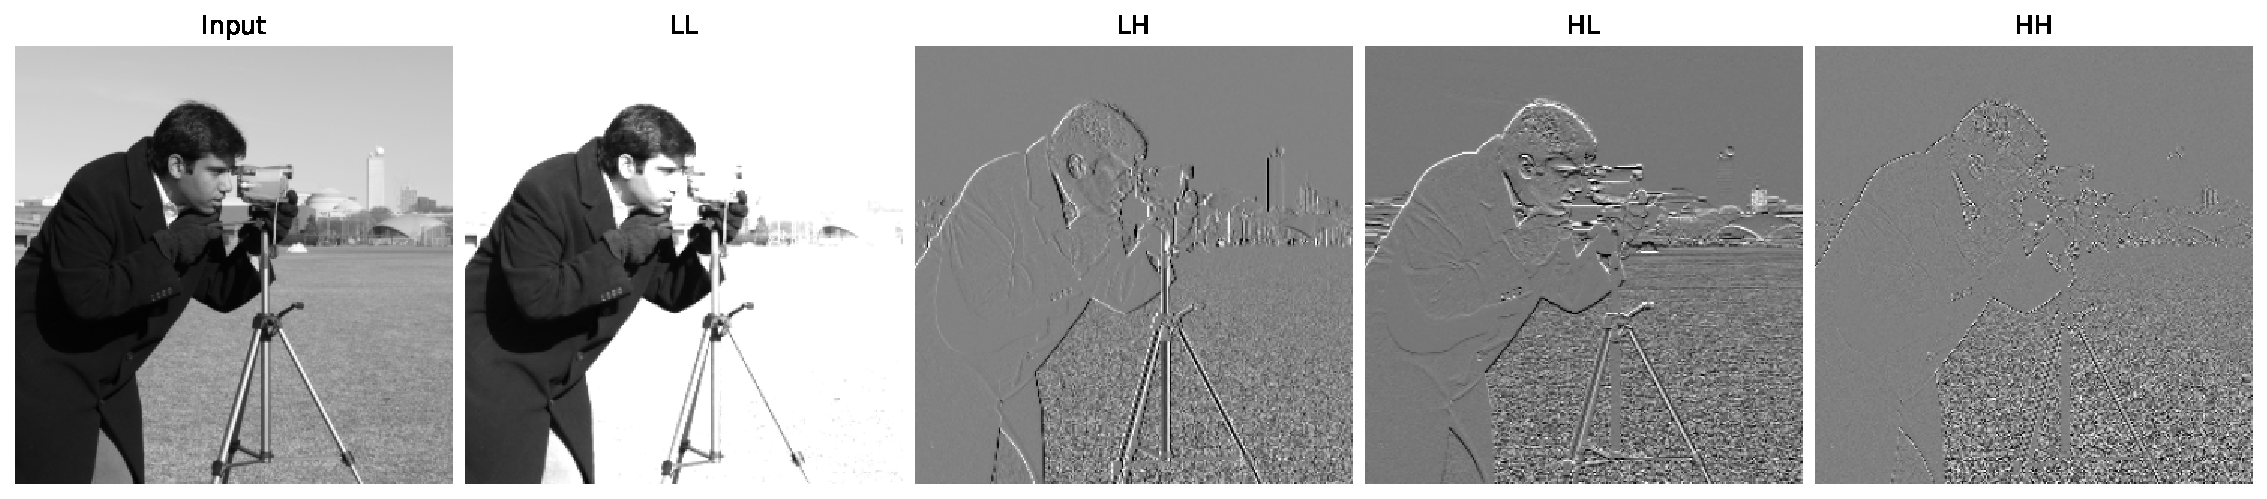
\includegraphics[width=0.98\textwidth]{haar_wavelet_real_image.pdf}
\caption{تجزیه موجک هار دوبعدی. نسبت انرژی ضرایب به تصویر \(\chthreeHaarEnergyRatio\) و بیشینه خطای
بازسازی \(\chthreeHaarReconstructionMaxAbs\) بود؛ این دو آزمون به‌ترتیب پارسوال و بازسازی کامل را
در پیاده‌سازی بررسی می‌کنند.}
\end{figure}

\subsection{موجک‌های فشرده دوبشی}
دوبشی نشان داد موجک‌های متعامد با تکیه‌گاه فشرده و درجات مختلف همواری و گشتاور محوشونده وجود دارند
\cite{daubechies1988wavelets}. افزایش گشتاورهای محوشونده نمایش چندجمله‌ای‌های کم‌درجه را در ضرایب
جزئیات صفر می‌کند، اما طول فیلتر و پیچیدگی مرزی افزایش می‌یابد.

\begin{definition}[گشتاور محوشونده]
موجک \(\psi\) دارای \(p\) گشتاور محوشونده است اگر
\begin{equation}
\int t^k\psi(t)dt=0,
\qquad k=0,\dots,p-1.
\end{equation}
\end{definition}

اگر تابع در یک ناحیه با چندجمله‌ای درجه کمتر از \(p\) تقریب‌پذیر باشد، ضرایب موجک ریزمقیاس در آن ناحیه
کوچک‌اند؛ ضرایب بزرگ نزدیک تکینگی‌ها و لبه‌ها متمرکز می‌شوند. این اساس تنکی موجک در فشرده‌سازی و حذف
نویز است.

\section{موجک دوبعدی و محدودیت جهت}

موجک جدایی‌پذیر دوبعدی چهار زیرباند تولید می‌کند:
\begin{align}
LL&=\phi(x)\phi(y),&
LH&=\phi(x)\psi(y),\\
HL&=\psi(x)\phi(y),&
HH&=\psi(x)\psi(y).
\end{align}
این ساختار برای جزئیات افقی، عمودی و قطری مناسب است، اما جهت‌های محدود دارد. برای تصویرهایی که در هر
مقیاس در امتداد منحنی‌های نرم تکینگی دارند، موجک‌های ایزوتروپیک بهینه نیستند.

\section{فیلتر جهت‌پذیر و هرم جهت‌پذیر}

فیلتر جهت‌پذیر را می‌توان در هر زاویه از ترکیب خطی تعداد محدودی فیلتر پایه ساخت. برای نمونه مشتق مرتبه اول
گاوسی در جهت \(\theta\):
\begin{equation}
G_\theta=\cos\theta\,G_x+\sin\theta\,G_y.
\label{eq:steer-first}
\end{equation}
این رابطه از مشتق جهتی
\begin{equation}
\partial_\theta=\cos\theta\partial_x+\sin\theta\partial_y
\end{equation}
می‌آید. \lr{Freeman--Adelson} نظریه عمومی طراحی و استفاده فیلترهای جهت‌پذیر را ارائه کردند
\cite{freeman1991steerable}. هرم جهت‌پذیر \lr{Simoncelli} نمایش چندمقیاسی، چندجهتی و بیش‌کامل با
شیفت‌پذیری بهتر می‌سازد \cite{simoncelli1992shiftable,simoncelli1995pyramid}.

\begin{keybox}[پایه در برابر چارچوب]
پایه هر سیگنال را با ضرایب یکتا نمایش می‌دهد. چارچوب می‌تواند افزونه باشد، اما کران‌های پایدار دارد:
\begin{equation}
A\norm f_2^2\le\sum_k|\inner f{\phi_k}|^2\le B\norm f_2^2.
\end{equation}
افزونگی می‌تواند پایداری نسبت به انتقال، جهت و حذف ضرایب را بهبود دهد، به بهای حافظه و ضرایب غیر یکتا.
\end{keybox}

\section{Curvelet و قانون مقیاس سهموی}

برای اشیای دوبعدی که بیرون از لبه‌های \(C^2\) هموارند، موجک‌های ایزوتروپیک لبه خمیده را با تعداد زیادی
ضریب نمایش می‌دهند. \lr{Curvelet}ها عناصر کشیده و جهت‌دار با قانون
\begin{equation}
\text{width}\approx(\text{length})^2
\end{equation}
دارند. در مقیاس \(2^{-j}\)، طول تقریبی \(2^{-j/2}\) و عرض \(2^{-j}\) است. کاندس و دونوهو نشان دادند
چارچوب‌های curvelet برای تکینگی‌های لبه‌ای \(C^2\) تقریب تنک نزدیک بهینه فراهم می‌کنند
\cite{candes2004curvelet}.

\begin{remark}
برتری یک تبدیل مطلق نیست. موجک برای تکینگی نقطه‌ای و ساختارهای جدایی‌پذیر عالی است؛ curvelet برای
لبه‌های خمیده؛ گابور برای بافت باریک‌باند؛ و تبدیل آموخته‌شده برای توزیع خاص داده. انتخاب باید بر اساس
مدل هندسی و وظیفه باشد.
\end{remark}

\section{تبدیل پراکنده‌سازی: موجک، غیرخطی و ناوردایی}

تبدیل پراکنده‌سازی \lr{Mallat} زنجیره‌ای از کانولوشن موجکی، قدرمطلق و میانگین‌گیری می‌سازد
\cite{mallat2012scattering}. برای مسیر \(p=(\lambda_1,\dots,\lambda_m)\):
\begin{equation}
\begin{aligned}
U[\emptyset]x&=x,\\
U[(p,\lambda)]x&=\left|U[p]x*\psi_{\lambda}\right|.
\end{aligned}
\end{equation}
و ضریب پراکنده‌سازی در مقیاس \(2^J\):
\begin{equation}
S_J[p]x=U[p]x*\phi_J.
\end{equation}

\begin{proposition}[غیرانبساطی‌بودن قدرمطلق]
برای اعداد مختلط \(a,b\):
\begin{equation}
\big||a|-|b|\big|\le|a-b|.
\end{equation}
پس عملگر قدرمطلق در \(L^2\) غیرانبساطی است.
\end{proposition}

اگر بانک موجک یک چارچوب فشرده/سفت مناسب باشد، زنجیره پراکنده‌سازی انرژی را کنترل می‌کند، نسبت به انتقال
در مقیاس میانگین‌گیری ناوردا و نسبت به تغییرشکل‌های کوچک لیپشیتس پایدار است. این معماری، پیش از یادگیری
عمیق مدرن، ساختاری شبیه شبکه کانولوشنی داشت؛ تفاوت آن است که فیلترها از تحلیل هارمونیک تعیین می‌شوند و
قضایای پایداری صریح‌اند.

\section{از فیلتر ثابت تا فیلتر آموختنی}

\subsection{کانولوشن شبکه عصبی همچنان یک عملگر محلی است}
برای کانال‌های ورودی و خروجی:
\begin{equation}
y_c[\vect n]=\sigma\left(\sum_{d=1}^{C_{\rm in}}h_{c,d}\star x_d[\vect n]+b_c\right).
\end{equation}
پیش از غیرخطی، هر جفت کانال یک فیلتر LSI است. اما ترکیب غیرخطی، تغییر کانال، نرمال‌سازی و زیرنمونه‌برداری
کل شبکه را عموماً نه خطی و نه انتقال‌ناوردا می‌کند.

\subsection{هم‌وردایی انتقال و زیرنمونه‌برداری}
کانولوشن با انتقال جابه‌جا می‌شود، اما زیرنمونه‌برداری برای انتقال‌های نامضرب گام چنین نیست. مقاله
\lr{Zhang} نشان داد قراردادن پایین‌گذر پیش از pooling یا کانولوشن گام‌دار می‌تواند ثبات انتقال و حتی دقت و
مقاومت را بهبود دهد \cite{zhang2019shift}.

\begin{figure}[H]
\centering
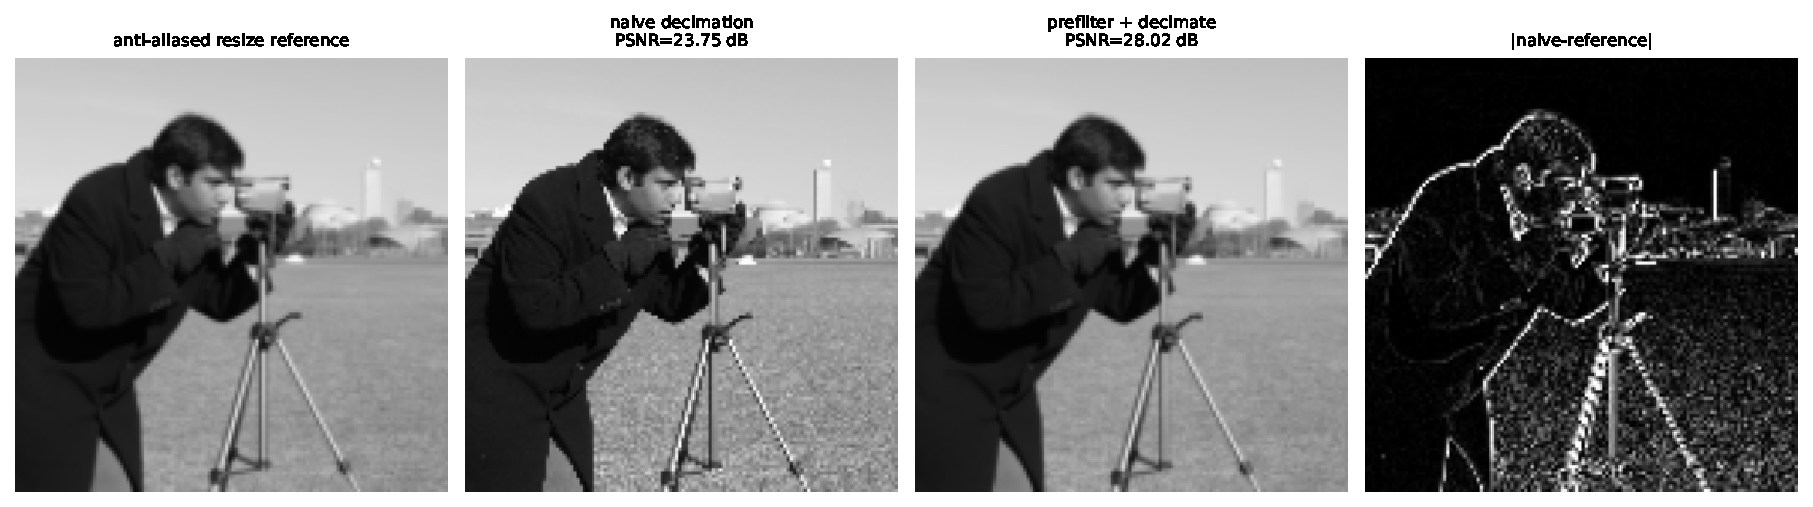
\includegraphics[width=0.95\textwidth]{antialias_real_downsampling.pdf}
\caption{کاهش اندازه چهاربرابری یک عکس واقعی. نسبت به مرجع بازنمونه‌برداری ضدعلیاس، PSNR کاهش نرخ خام
\(\chthreeNaiveDownsamplePsnr\) dB و پیش‌فیلترشده \(\chthreePrefilterDownsamplePsnr\) dB است.
پیش‌فیلتر جزئیات غیرقابل‌نمایش را حذف می‌کند؛ پس از زیرنمونه‌برداری دیگر بازگردانی علیاس ممکن نیست.}
\end{figure}

\subsection{مدل مولد بدون علیاس}
\lr{StyleGAN3} منشأ «چسبیدن بافت به مختصات تصویر» را در پردازش سیگنال نامناسب و تولید فرکانس‌های خارج
از باند میان لایه‌ها تحلیل کرد. با تفسیر سیگنال‌ها به‌عنوان توابع پیوسته و کنترل پایین‌گذر، هم‌وردایی زیرپیکسلی
به انتقال و چرخش بهبود یافت \cite{karras2021aliasfree}. پیام آموزشی مهم این است: شبکه عمیق قوانین
نمونه‌برداری را لغو نمی‌کند.

\section{سوگیری طیفی شبکه‌های عصبی}

شبکه‌های ReLU و MLPهای متعارف در آموزش گرادیانی اغلب مؤلفه‌های کم‌فرکانس را زودتر از پرفرکانس یاد
می‌گیرند. \lr{Rahaman et al.} این پدیده را سوگیری طیفی تحلیل کردند \cite{rahaman2019spectral}.
این رفتار می‌تواند به همواری و تعمیم کمک کند، ولی برای بازنمایی جزئیات ریز، میدان موج یا تصویر با بافت
پرفرکانس مانع باشد.

\subsection{Fourier Features}
نگاشت
\begin{equation}
\gamma(\vect x)=
[\cos(2\pi B\vect x),\sin(2\pi B\vect x)]
\end{equation}
به MLP دسترسی صریح به پایه‌های فرکانسی می‌دهد. \lr{Tancik et al.} نشان دادند این نگاشت پهنای باند کرنل
مؤثر شبکه را قابل تنظیم و یادگیری توابع پرفرکانس کم‌بعد را آسان می‌کند \cite{tancik2020fourier}.

\begin{figure}[H]
\centering
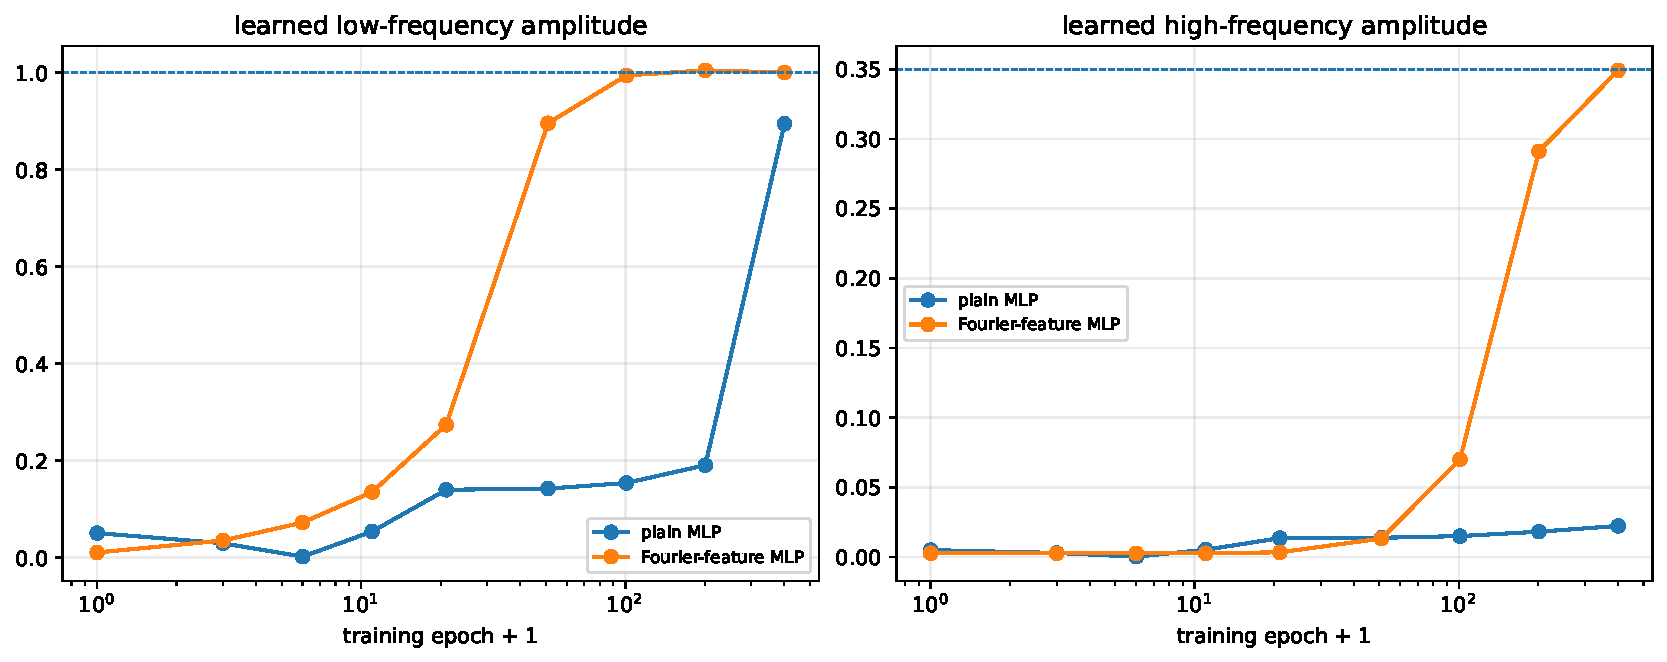
\includegraphics[width=0.88\textwidth]{spectral_bias_fourier_features.pdf}
\caption{آزمایش بازتولیدپذیر روی تابعی شامل فرکانس پایه و مؤلفه ده‌برابر. پس از ۴۰۰ گام، دامنه پرفرکانس
آموخته‌شده توسط MLP ساده \(\chthreePlainHighAmpFinal\) و توسط MLP با Fourier Features برابر
\(\chthreeFourierHighAmpFinal\) شد؛ مقدار حقیقی ۰٫۳۵ است. خطای نهایی نیز از
\(\chthreePlainLossFinal\) به \(\chthreeFourierLossFinal\) کاهش یافت.}
\end{figure}

\subsection{SIREN}
\lr{SIREN} از فعال‌ساز سینوسی و مقداردهی اولیه متناسب استفاده می‌کند و برای نمایش ضمنی تصویر، ویدئو،
میدان موج و مشتق‌ها طراحی شده است \cite{sitzmann2020siren}. فرکانس در اینجا فقط ابزار تحلیل خروجی نیست؛
در خود معماری قرار گرفته است.

\subsection{Fourier Neural Operator}
\lr{FNO} نگاشت میان فضاهای تابعی را با پارامتردهی کرنل انتگرالی در حوزه فوریه می‌آموزد:
\begin{equation}
(\op K_\theta v)(x)=\FT^{-1}\left(R_\theta(k)\FT v(k)\right)(x),
\end{equation}
معمولاً با تعداد محدودی مد. هدف اصلی حل خانواده‌ای از PDEها است، نه صرفاً فیلترکردن تصویر
\cite{li2021fno}. این مثال نشان می‌دهد قضیه کانولوشن از پردازش کلاسیک به یادگیری عملگر منتقل شده است.

\begin{futurebox}
دهه آینده نه «جایگزینی فوریه با شبکه» و نه «بازگشت صرف به فیلتر کلاسیک» است. مسیر قوی‌تر، معماری‌هایی
است که ساختارهای اثبات‌شده ــ تقارن، باند، مقیاس، پایداری و عملگر فیزیکی ــ را در مدل آموختنی وارد کنند.
نمونه‌ها شامل شبکه‌های مشتق گاوسی هم‌وردا با مقیاس، مدل‌های بدون علیاس، neural operatorها، نمایش‌های ضمنی
دوره‌ای و تبدیل‌های موجکی آموختنی است \cite{lindeberg2020scale,karras2021aliasfree,li2021fno,sitzmann2020siren}.
\end{futurebox}

\section{آزمایش محوری فصل: ممیزی یک خط لوله فرکانسی روی داده واقعی}

هدف آزمایش، کسب یک عدد بهتر نیست؛ آزمون سازگاری نظریه، پیاده‌سازی و گزارش است. داده اصلی دو عکس واقعی
استاندارد از بسته \lr{scikit-image} است \cite{vanderwalt2014skimage}. مراحل:
\begin{enumerate}
\item ساخت کرنل گاوسی و مقایسه کانولوشن مستقیم و FFT با مرز یکسان؛
\item آزمون قطری‌شدن ماتریس دوری؛
\item بازسازی دامنه/فاز و گزارش SSIM؛
\item مقایسه شرط‌های مرزی در نوار مرز؛
\item آزمون نیم‌گروه گاوسی؛
\item ساخت هرم لاپلاسی و آزمون بازسازی؛
\item ساخت موجک هار و آزمون انرژی/بازسازی؛
\item کاهش نرخ با و بدون ضدعلیاس؛
\item بازتولید یک آزمایش کوچک سوگیری طیفی و Fourier Features؛
\item ذخیره همه بذرها، نسخه‌ها و خروجی عددی در CSV.
\end{enumerate}

\subsection{جدول نتایج واقعی اجرای همراه فصل}

\begin{longtable}{p{0.39\textwidth}p{0.18\textwidth}p{0.34\textwidth}}
\toprule
آزمون & نتیجه & تفسیر\\
\midrule
\endfirsthead
\toprule
آزمون & نتیجه & تفسیر\\
\midrule
\endhead
نسبت بخش خارج قطر \(FCF^*\) & \(\chthreeDftOffdiagRatio\) & قطری‌شدن تا دقت گردکردن تأیید شد.\\
FFT در برابر کانولوشن مستقیم با مرز صفر & \(\chthreeFftVsZeroSpatialRelLTwo\) & دو پیاده‌سازی از نظر مدل یکسان‌اند.\\
خطای مرز انعکاسی & \(\chthreeBoundaryReflectRmse\) & از صفر و دوری بسیار کمتر بود؛ وابسته به مرجع انتخابی.\\
نیم‌گروه فضای مقیاس & \(\chthreeSemigroupRelativeError\) & اختلاف از گسسته‌سازی و قطع کرنل است.\\
بازسازی هرم لاپلاسی & \(\chthreeLaplacianReconstructionMaxAbs\) & بازسازی جبری در دقت ماشین.\\
بازسازی هار & \(\chthreeHaarReconstructionMaxAbs\) & بانک فیلتر متعامد درست پیاده‌سازی شده است.\\
PSNR کاهش نرخ خام & \(\chthreeNaiveDownsamplePsnr\) dB & علیاس و خطای نمونه‌برداری قابل مشاهده است.\\
PSNR پیش‌فیلترشده & \(\chthreePrefilterDownsamplePsnr\) dB & کنترل باند پیش از کاهش نرخ نتیجه را بهبود داد.\\
دامنه پرفرکانس MLP ساده & \(\chthreePlainHighAmpFinal\) & مؤلفه سریع در بودجه آموزش یاد گرفته نشد.\\
دامنه پرفرکانس Fourier Features & \(\chthreeFourierHighAmpFinal\) & نزدیک مقدار حقیقی ۰٫۳۵ شد.\\
\bottomrule
\end{longtable}

\begin{warningbox}
این نتایج برای اثبات برتری عمومی یک الگوریتم کافی نیستند. آن‌ها آزمون‌های واحد علمی‌اند: هر عدد باید یک
خاصیت مشخص را تأیید یا رد کند. برای مقاله، تصاویر بیشتر، تکرار آماری، کنترل پارامترها و تحلیل حساسیت لازم است.
\end{warningbox}

\section{کد هسته آزمایش‌ها}

\paragraph{آزمون سازگاری کانولوشن مستقیم و FFT با مرز صفر.}
\begin{LTR}
\begin{lstlisting}
import numpy as np
from scipy import signal


def gaussian_kernel(size: int, sigma: float) -> np.ndarray:
    axis = np.arange(-(size // 2), size // 2 + 1)
    xx, yy = np.meshgrid(axis, axis, indexing="xy")
    kernel = np.exp(-(xx**2 + yy**2) / (2.0 * sigma**2))
    return kernel / kernel.sum()


def relative_l2(a: np.ndarray, b: np.ndarray) -> float:
    return float(np.linalg.norm(a - b) / max(np.linalg.norm(a), 1e-15))


kernel = gaussian_kernel(31, 4.0)
y_direct = signal.convolve2d(
    image, kernel, mode="same", boundary="fill", fillvalue=0.0
)
y_fft = signal.fftconvolve(image, kernel, mode="same")
assert relative_l2(y_direct, y_fft) < 1e-12
\end{lstlisting}
\end{LTR}

\paragraph{آزمون عددی الحاقی برای عملگر کانولوشن.}
\begin{LTR}
\begin{lstlisting}
def adjoint_test(A, AT, shape, seed=1405):
    rng = np.random.default_rng(seed)
    x = rng.normal(size=shape)
    z = rng.normal(size=shape)
    lhs = np.vdot(A(x), z)
    rhs = np.vdot(x, AT(z))
    denominator = max(1.0, abs(lhs), abs(rhs))
    return float(abs(lhs - rhs) / denominator)


error = adjoint_test(blur, blur_adjoint, image.shape)
assert error < 1e-10
\end{lstlisting}
\end{LTR}

\paragraph{آزمون نیم‌گروه گاوسی.}
\begin{LTR}
\begin{lstlisting}
from scipy import ndimage

sigma1, sigma2 = 1.7, 2.9
left = ndimage.gaussian_filter(
    ndimage.gaussian_filter(image, sigma1, mode="reflect"),
    sigma2,
    mode="reflect",
)
right = ndimage.gaussian_filter(
    image,
    np.sqrt(sigma1**2 + sigma2**2),
    mode="reflect",
)
error = relative_l2(left, right)
print(error)
\end{lstlisting}
\end{LTR}

\section{چک‌لیست صحت پیاده‌سازی}

\begin{enumerate}
\item مجموع کرنل پایین‌گذر یک و مجموع کرنل مشتق صفر است؟
\item مرکز کرنل برای اندازه زوج چگونه تعریف شده است؟
\item عملیات کد کانولوشن است یا همبستگی؟
\item شرط مرزی در مدل، کد و مقایسه یکسان است؟
\item پد برای کانولوشن خطی به اندازه کافی بزرگ است؟
\item ترتیب \lr{fftshift/ifftshift} با محل مرکز کرنل سازگار است؟
\item نرمال‌سازی DFT و IDFT در پارسوال لحاظ شده است؟
\item برای تصویر حقیقی، تقارن هرمیتی رعایت شده است؟
\item واحد محور فرکانس مشخص است؟
\item پیش از کاهش نرخ پایین‌گذر مناسب اعمال شده است؟
\item آزمون بازسازی کامل برای هرم/موجک وجود دارد؟
\item آزمون الحاقی برای عملگر و الحاقی آن وجود دارد؟
\item مقایسه زمان پس از warm-up و با چند تکرار انجام شده است؟
\item نسخه NumPy/SciPy/PyTorch، بذر و نوع داده ثبت شده است؟
\end{enumerate}

\section{تمرین‌های اثباتی}

\begin{enumerate}
\item نشان دهید اگر \(h\in\ell^1\)، عملگر کانولوشن روی \(\ell^2\) کراندار است و
\(\norm{T_h}_{2\to2}\le\norm h_1\). سپس با DTFT نشان دهید نرم دقیق برابر
\(\esssup_\omega|H(e^{i\omega})|\) است.
\item شرط لازم پایداری BIBO سامانه گسسته LTI را با ورودی مناسب اثبات کنید.
\item برای کرنل حقیقی، رابطه تقارن هرمیتی پاسخ فرکانسی را اثبات کنید. اگر کرنل حقیقی و زوج باشد چه نتیجه‌ای
برای فاز می‌گیرید؟
\item ثابت کنید کانولوشن با کرنل جدایی‌پذیر معادل دو کانولوشن یک‌بعدی است و نسبت پیچیدگی را برای
\(K=31\) محاسبه کنید.
\item ماتریس BCCB یک کانولوشن \(3\times3\) روی تصویر \(4\times4\) را صریح بسازید و با ضرب DFT
دوبعدی قطری‌بودن آن را نشان دهید.
\item رابطه تبدیل فوریه تغییر خطی مختصات \(f(Ax)\) را با تغییر متغیر اثبات کنید.
\item رابطه مشتق فوریه را با انتگرال‌گیری جزءبه‌جز و شروط مرزی دقیق اثبات کنید.
\item اصل عدم قطعیت \eqref{eq:uncertainty} را کامل کنید و شرط برابری را استخراج نمایید.
\item نشان دهید گاوسی تنها تابعی است که در نامساوی عدم قطعیت برابری می‌دهد، تا انتقال، مدولاسیون و مقیاس.
\item خاصیت نیم‌گروه گاوسی را یک بار با فوریه و یک بار با محاسبه مستقیم انتگرال اثبات کنید.
\item از معادله گرما نشان دهید انرژی \(\norm{L(\cdot;t)}_2^2\) با \(t\) غیرصعودی است:
\begin{equation}
\frac{d}{dt}\norm L_2^2=-2\norm{\nabla L}_2^2.
\end{equation}
\item رابطه steerability مرتبه دوم را برای \(G_{xx},G_{xy},G_{yy}\) استخراج کنید.
\item شرط بازسازی کامل بانک فیلتر دوکاناله را از تجزیه مؤلفه مطلوب و مؤلفه علیاس به دست آورید.
\item پارسوال موجک هار را مستقیماً برای یک بلوک \(2\times2\) اثبات کنید.
\item نشان دهید اگر موجک \(p\) گشتاور محوشونده داشته باشد، ضریب آن روی چندجمله‌ای درجه کمتر از \(p\)
صفر است.
\end{enumerate}

\section{تمرین‌های عددی و مهندسی}

\begin{enumerate}
\item یک کرنل تاری حرکت بسازید و پاسخ اندازه و فاز آن را رسم کنید. جهت صفرهای طیف را با جهت حرکت توضیح دهید.
\item سه شرط مرزی را روی پنج تصویر واقعی و سه اندازه کرنل مقایسه کنید. خطا را جداگانه در نوار مرز و ناحیه
داخلی گزارش کنید.
\item آستانه اندازه کرنلی را که از آن FFT روی رایانه شما سریع‌تر می‌شود، برای تصاویر ۵۱۲، ۱۰۲۴ و ۲۰۴۸
پیکسل بیابید.
\item اثر float32 و float64 را بر آزمون قطری‌شدن، بازسازی هرم و آزمون الحاقی اندازه بگیرید.
\item فیلترهای جعبه‌ای، گاوسی و باتروورث را با پهنای نیم‌توان یکسان طراحی و حلقه‌زنی آن‌ها را مقایسه کنید.
\item از یک لبه مایل واقعی عکس بگیرید، ESF/LSF/MTF را محاسبه کنید و توضیح دهید چرا نتیجه شما آزمون رسمی
ISO نیست.
\item فضای مقیاس گاوسی را برای بافت طبیعی بسازید و تعداد اکسترمم/عبور صفر را با مقیاس اندازه‌گیری کنید.
\item هرم لاپلاسی را برای ترکیب چندباند دو عکس پیاده‌سازی کنید و اثر تعداد سطوح را تحلیل کنید.
\item موجک هار و یک موجک دوبشی را روی همان تصویر مقایسه کنید: انرژی ۱ درصد بزرگ‌ترین ضرایب چقدر است؟
\item یک تصویر با لبه منحنی بسازید و تنکی موجک و یک تبدیل جهت‌دار را از نظر منحنی خطای تقریب \(m\)-جمله‌ای
مقایسه کنید.
\item آزمایش سوگیری طیفی فصل را با ReLU، tanh و SIREN تکرار کنید. نتیجه را برحسب زمان و تعداد پارامتر گزارش کنید.
\item یک لایه stride-2 را با و بدون پایین‌گذر روی جابه‌جایی‌های زیرپیکسلی آزمایش و خطای هم‌وردایی تعریف کنید.
\end{enumerate}

\section{تمرین‌های خواندن مقاله}

برای هر مقاله، دانشجو باید یک صفحه شامل «مسئله»، «فرض ریاضی»، «قضیه/ادعا»، «آزمایش کلیدی» و «محدودیت»
تحویل دهد:
\begin{enumerate}
\item \lr{Cooley--Tukey (1965)}: الگوریتم دقیقاً چه تجزیه‌ای از اندازه \(N\) فرض می‌کند؟
\item \lr{Koenderink (1984)}: مفهوم ساختار تصویر در طول مقیاس چیست؟
\item \lr{Burt--Adelson (1983)}: چرا هرم لاپلاسی هم مکانی و هم فرکانسی موضعی است؟
\item \lr{Mallat (1989)}: پیوند MRA و بانک فیلتر چگونه ساخته می‌شود؟
\item \lr{Daubechies (1988)}: مصالحه تکیه‌گاه، تعامد و همواری چیست؟
\item \lr{Freeman--Adelson (1991)}: شرط جهت‌پذیری در حوزه زاویه چیست؟
\item \lr{Mallat (2012)}: ناوردایی و پایداری scattering دقیقاً نسبت به چه تبدیل‌هایی است؟
\item \lr{Zhang (2019)}: چرا پایین‌گذر ساده اگر نادرست وارد شبکه شود می‌تواند دقت را کم کند؟
\item \lr{Tancik et al. (2020)}: Fourier Features چگونه کرنل مؤثر شبکه را تغییر می‌دهد؟
\item \lr{Karras et al. (2021)}: تعریف سیگنال پیوسته در شبکه مولد چه خطای معماری را آشکار می‌کند؟
\end{enumerate}

\section{پرامپت پیشنهادی برای Codex}

\begin{workshopbox}[پروژه فصل سوم]
یک مخزن پژوهش‌پذیر Python بساز که تمام آزمایش‌های فصل سوم را روی حداقل پنج تصویر واقعی اجرا کند.
ساختار شامل \lr{src/}، \lr{tests/}، \lr{configs/}، \lr{outputs/} و \lr{report/} باشد. الزامات:
\begin{enumerate}
\item کانولوشن مستقیم، جدایی‌پذیر و FFT با شرط‌های مرزی صفر، دوری و انعکاسی؛
\item آزمون خودکار کانولوشن، پارسوال، تقارن هرمیتی، قطری‌شدن BCCB و الحاقی؛
\item تولید پاسخ مکانی و فرکانسی فیلترهای جعبه‌ای، گاوسی، باتروورث، مشتق گاوسی و غیرشارپ؛
\item برآورد آموزشی MTF از لبه مایل با هشدار روشن درباره عدم انطباق رسمی با ISO؛
\item فضای مقیاس، هرم گاوسی/لاپلاسی و بازسازی کامل؛
\item موجک هار از صفر و دست‌کم یک موجک کتابخانه‌ای با آزمون انرژی؛
\item آزمایش anti-aliasing قبل از downsampling و معیار shift consistency؛
\item آزمایش spectral bias برای MLP معمولی، Fourier Features و SIREN با بذر ثابت؛
\item ذخیره CSV شامل زمان، خطا، PSNR/SSIM، نسخه کتابخانه و سخت‌افزار؛
\item تولید خودکار شکل‌های PDF و قطعه LaTeX جدول نتایج؛
\item هیچ عدد ساختگی، تصویر placeholder یا نتیجه hard-coded مجاز نیست؛ هر خروجی باید از اجرای واقعی ساخته شود.
\end{enumerate}
\end{workshopbox}

\section{تقسیم فصل به ویدئوهای پانزده‌دقیقه‌ای}

\begin{videobox}
\begin{longtable}{p{0.07\textwidth}p{0.34\textwidth}p{0.49\textwidth}}
\toprule
بخش & عنوان ویدئو & خروجی قابل تحویل\\
\midrule
\endfirsthead
\toprule
بخش & عنوان ویدئو & خروجی قابل تحویل\\
\midrule
\endhead
1 & چرا فیلتر یک ماسک نیست؟ & تعریف عملگر، دامنه، مرز و واحد.\\
2 & انتقال و دلتا & تفاوت دلتا گسسته و توزیع دیراک.\\
3 & اثبات نمایش کانولوشنی & اثبات کامل قضیه LSI گسسته.\\
4 & پایداری و نامساوی یانگ & کران بهره و تفسیر BIBO.\\
5 & جدایی‌پذیری و همسانگردی & کاهش پیچیدگی گاوسی.\\
6 & Toeplitz و BCCB & ساخت ماتریس یک مثال کوچک.\\
7 & شرط مرزی & آزمایش واقعی صفر، دوری و انعکاس.\\
8 & الحاقی کانولوشن & آزمون inner-product.\\
9 & فوریه پیوسته & قرارداد، وارون‌سازی و ریمان ـ لبگ.\\
10 & پلانشرل و کانولوشن & اثبات و کران نرم عملگر.\\
11 & تابع ویژه سینوسی & پاسخ فرکانسی به‌عنوان مقدار ویژه.\\
12 & دامنه و فاز & آزمایش بازسازی عکس واقعی.\\
13 & DFT ماتریسی & تعامد و پارسوال گسسته.\\
14 & قطری‌شدن کانولوشن دوری & اثبات و آزمون عددی.\\
15 & FFT & استخراج radix-2 و پیچیدگی.\\
16 & نشت طیفی & پنجره، پد صفر و تفکیک واقعی.\\
17 & طراحی پایین‌گذر & جعبه‌ای، گاوسی و باتروورث.\\
18 & گیبس و تیزکردن & مصالحه حوزه مکان و فرکانس.\\
19 & مشتق و لاپلاسین & تقویت نویز و مشتق گاوسی.\\
20 & PSF/OTF/MTF & زنجیره انتقال کنتراست.\\
21 & لبه مایل ISO 12233 & ESF، LSF، MTF و محدودیت آزمایش.\\
22 & وارون‌سازی و صفرهای طیف & بدوضعی در پایه فوریه.\\
23 & اصول فضای مقیاس & یکتایی گاوسی و نیم‌گروه.\\
24 & معادله گرما & اثبات و اصل بیشینه.\\
25 & هرم گاوسی و لاپلاسی & ساخت و بازسازی کامل.\\
26 & عدم قطعیت و STFT & مصالحه مکان ـ فرکانس.\\
27 & فیلترهای گابور & بانک جهت و فاز موضعی.\\
28 & موجک پیوسته & پذیرش و بازسازی.\\
29 & MRA و بانک فیلتر & معادله پالایش و زیرفضاها.\\
30 & هار و دوبشی & گشتاور محوشونده و تنکی.\\
31 & هرم جهت‌پذیر و curvelet & قانون مقیاس سهموی.\\
32 & scattering & ناوردایی، پایداری و پل به CNN.\\
33 & ضدعلیاسینگ شبکه & stride، pooling و StyleGAN3.\\
34 & سوگیری طیفی & Rahaman، Fourier Features و SIREN.\\
35 & Fourier Neural Operator & یادگیری نگاشت میان فضاهای تابعی.\\
36 & آزمایش محوری و گزارش & اجرای کامل، جدول و ممیزی فرض‌ها.\\
\bottomrule
\end{longtable}
\end{videobox}

\section{خلاصه دقیق فصل}

\begin{enumerate}
\item هر سامانه خطی انتقال‌ناوردا با پاسخ ضربه و کانولوشن مشخص می‌شود، مشروط به فضای تابعی و پیوستگی مناسب.
\item نامساوی یانگ کران پایداری کانولوشن را می‌دهد و نرم \(\ell^1\) کرنل بهره بدترین‌حالت را کنترل می‌کند.
\item کانولوشن، همبستگی و عملیات موسوم به convolution در چارچوب‌های عمیق باید از هم تفکیک شوند.
\item شرط مرزی بخشی از مدل پیشرو است؛ صفر، دوری و انعکاس خروجی‌های متفاوت و ماتریس‌های متفاوت می‌سازند.
\item ماتریس کانولوشن دوری BCCB در پایه DFT قطری است؛ این ارتباط جبر خطی و تحلیل فرکانسی را یکی می‌کند.
\item پلانشرل انرژی را میان مکان و فرکانس حفظ می‌کند و قضیه کانولوشن فیلتر LSI را به ضرب نقطه‌ای تبدیل می‌کند.
\item سینوس‌های مختلط تابع ویژه سامانه انتقال‌ناوردا هستند؛ پاسخ فرکانسی مقدار ویژه وابسته به فرکانس است.
\item فاز هم‌ترازی مکانی و دامنه توزیع انرژی طیفی را حمل می‌کند؛ حذف هرکدام اطلاعات متفاوتی را نابود می‌کند.
\item DFT نمایش تناوبی داده محدود است و FFT فقط سازمان محاسبه را تغییر می‌دهد، نه تعریف تبدیل را.
\item پنجره‌گذاری موجب کانولوشن طیفی و نشت می‌شود؛ پد صفر اطلاعات جدید ایجاد نمی‌کند.
\item فیلتر ایده‌آل گذار تیز ولی کرنل نامتناهی و حلقه‌زنی گیبس دارد؛ طراحی همواره مصالحه است.
\item PSF پاسخ نقطه، OTF تبدیل مختلط آن و MTF اندازه OTF است؛ MTF فاز را حذف می‌کند.
\item روش لبه مایل از ESF به LSF و سپس MTF می‌رسد، اما اجرای آموزشی معادل آزمون رسمی ISO نیست.
\item افت پاسخ فرکانسی به معنای مقادیر منفرد کوچک و حساسیت وارون‌سازی به نویز است.
\item فضای مقیاس خطی تحت اصول ساختاری به گاوسی می‌رسد و با معادله گرما و اصل بیشینه مرتبط است.
\item هرم لاپلاسی نمایش چندباند موضعی و قابل بازسازی است؛ تعداد کل نمونه‌های هرم گاوسی دوبعدی حدود \(4/3\) تصویر است.
\item اصل عدم قطعیت مانع تمرکز دلخواه هم‌زمان در مکان و فرکانس است؛ گاوسی حد بهینه را می‌سازد.
\item موجک با مقیاس تطبیقی، MRA و بانک فیلتر، نمایش مکان ـ مقیاس فراهم می‌کند؛ گشتاور محوشونده تنکی را توضیح می‌دهد.
\item فیلتر جهت‌پذیر، هرم steerable و curvelet محدودیت جهت موجک جدایی‌پذیر را هدف می‌گیرند.
\item scattering ساختار موجکی را با غیرخطی غیرانبساطی ترکیب می‌کند و قضایای ناوردایی/پایداری دارد.
\item شبکه عمیق قوانین نمونه‌برداری را حذف نمی‌کند؛ ضدعلیاسینگ و کنترل باند برای هم‌وردایی ضروری است.
\item سوگیری طیفی MLP، Fourier Features، SIREN و FNO نشان می‌دهند تحلیل فوریه همچنان در قلب مدل‌های جدید است.
\end{enumerate}

\section{واژگان کلیدی فصل}

\begin{longtable}{>{\bfseries}p{0.28\textwidth}p{0.64\textwidth}}
\toprule
واژه & تعریف دقیق\\
\midrule
\endfirsthead
\toprule
واژه & تعریف دقیق\\
\midrule
\endhead
سامانه LSI & عملگر خطی که با انتقال جابه‌جا می‌شود و با پاسخ ضربه مشخص می‌گردد.\\
پاسخ ضربه & خروجی سامانه به دلتا؛ کرنل کانولوشن سامانه LSI.\\
همبستگی & مقایسه یک الگو با انتقال‌های سیگنال؛ معادل کانولوشن با کرنل مزدوج ـ وارونه.\\
Toeplitz & ماتریسی با درایه ثابت روی هر قطر؛ نمایش کانولوشن خطی محدود.\\
BCCB & ماتریس بلوکی دوری با بلوک‌های دوری؛ نمایش کانولوشن دوری دوبعدی.\\
الحاقی & عملگری که \(\inner{Ax}{z}=\inner{x}{A^*z}\) را برقرار می‌کند.\\
پلانشرل & واحدی‌بودن تبدیل فوریه روی \(L^2\) و حفظ انرژی تا ضریب قرارداد.\\
پاسخ فرکانسی & مقدار ویژه سامانه LSI برای نمایی مختلط هر فرکانس.\\
DFT & نمایش متناهی در پایه نمایی‌های تناوبی گسسته.\\
FFT & خانواده الگوریتم‌های سریع محاسبه DFT، نه تبدیل متفاوت.\\
نشت طیفی & پخش انرژی میان فرکانس‌ها در اثر مشاهده محدود/پنجره‌گذاری.\\
PSF & پاسخ سامانه تصویربرداری به نقطه.\\
OTF & تبدیل فوریه مختلط PSF.\\
MTF & اندازه OTF و انتقال کنتراست برحسب فرکانس.\\
فضای مقیاس & خانواده نمایش‌های تصویر با پارامتر تفکیک/مقیاس و اصول سازگاری ساختاری.\\
نیم‌گروه & ترکیب دو هموارسازی با پارامترهای \(t_1,t_2\) معادل پارامتر \(t_1+t_2\).\\
هرم لاپلاسی & نمایش اختلاف سطح گاوسی و پیش‌بینی بازگسترش‌یافته سطح درشت‌تر.\\
اصل عدم قطعیت & کران پایین حاصل‌ضرب پراکندگی مکان و فرکانس.\\
موجک & اتم میانگین‌صفر موضعی‌شده که با انتقال و مقیاس خانواده می‌سازد.\\
MRA & دنباله تو در توی زیرفضاهای تقریب که موجک و بانک فیلتر را صورت‌بندی می‌کند.\\
گشتاور محوشونده & صفر بودن انتگرال موجک ضرب در چندجمله‌ای‌های کم‌درجه.\\
چارچوب & خانواده احتمالاً افزونه با کران‌های پایدار تحلیل.\\
جهت‌پذیری & ساخت پاسخ فیلتر در زاویه دلخواه از ترکیب محدود فیلترهای پایه.\\
Scattering & زنجیره موجک، قدرمطلق و میانگین با ناوردایی و پایداری کنترل‌شده.\\
سوگیری طیفی & گرایش فرایند آموزش شبکه به یادگیری زودتر مؤلفه‌های کم‌فرکانس.\\
Fourier Features & نگاشت ورودی به سینوس و کسینوس برای کنترل پهنای باند نمایش شبکه.\\
Neural Operator & مدل آموختنی نگاشت میان فضاهای تابعی، نه فقط بردارهای با بعد ثابت.\\
\bottomrule
\end{longtable}
% === END CHAPTER CONTENT ===

\backmatter
\renewcommand{\bibname}{منابع علمی، کتاب‌ها، استانداردها و مقالات فصل سوم}
\addcontentsline{toc}{chapter}{منابع علمی، کتاب‌ها، استانداردها و مقالات فصل سوم}
\begin{thebibliography}{99}
\begin{LTR}

\bibitem{bracewell2000fourier}
R. N. Bracewell,
\emph{The Fourier Transform and Its Applications}, 3rd ed., McGraw--Hill, 2000.

\bibitem{oppenheim1999dsp}
A. V. Oppenheim, R. W. Schafer, and J. R. Buck,
\emph{Discrete-Time Signal Processing}, 2nd ed., Prentice Hall, 1999.

\bibitem{mallat2009wavelet}
S. Mallat,
\emph{A Wavelet Tour of Signal Processing: The Sparse Way}, 3rd ed., Academic Press, 2009.

\bibitem{daubechies1992ten}
I. Daubechies,
\emph{Ten Lectures on Wavelets}, SIAM, 1992.

\bibitem{gonzalez2018dip}
R. C. Gonzalez and R. E. Woods,
\emph{Digital Image Processing}, 4th ed., Pearson, 2018.

\bibitem{szeliski2022cv}
R. Szeliski,
\emph{Computer Vision: Algorithms and Applications}, 2nd ed., Springer, 2022.

\bibitem{hansen2006deblurring}
P. C. Hansen, J. G. Nagy, and D. P. O'Leary,
\emph{Deblurring Images: Matrices, Spectra, and Filtering}, SIAM, 2006.

\bibitem{cooley1965fft}
J. W. Cooley and J. W. Tukey,
``An Algorithm for the Machine Calculation of Complex Fourier Series,''
\emph{Mathematics of Computation}, vol. 19, no. 90, pp. 297--301, 1965,
doi: 10.1090/S0025-5718-1965-0178586-1.

\bibitem{gabor1946communication}
D. Gabor,
``Theory of Communication. Part 1: The Analysis of Information,''
\emph{Journal of the Institution of Electrical Engineers--Part III}, vol. 93, no. 26,
pp. 429--441, 1946, doi: 10.1049/ji-3-2.1946.0074.

\bibitem{koenderink1984structure}
J. J. Koenderink,
``The Structure of Images,''
\emph{Biological Cybernetics}, vol. 50, pp. 363--370, 1984,
doi: 10.1007/BF00336961.

\bibitem{lindeberg1994scale}
T. Lindeberg,
\emph{Scale-Space Theory in Computer Vision}, Kluwer Academic Publishers, 1994.

\bibitem{lindeberg1998automatic}
T. Lindeberg,
``Feature Detection with Automatic Scale Selection,''
\emph{International Journal of Computer Vision}, vol. 30, pp. 79--116, 1998.

\bibitem{burt1983laplacian}
P. J. Burt and E. H. Adelson,
``The Laplacian Pyramid as a Compact Image Code,''
\emph{IEEE Transactions on Communications}, vol. 31, no. 4, pp. 532--540, 1983,
doi: 10.1109/TCOM.1983.1095851.

\bibitem{mallat1989mra}
S. G. Mallat,
``A Theory for Multiresolution Signal Decomposition: The Wavelet Representation,''
\emph{IEEE Transactions on Pattern Analysis and Machine Intelligence}, vol. 11, no. 7,
pp. 674--693, 1989.

\bibitem{daubechies1988wavelets}
I. Daubechies,
``Orthonormal Bases of Compactly Supported Wavelets,''
\emph{Communications on Pure and Applied Mathematics}, vol. 41, no. 7,
pp. 909--996, 1988, doi: 10.1002/cpa.3160410705.

\bibitem{freeman1991steerable}
W. T. Freeman and E. H. Adelson,
``The Design and Use of Steerable Filters,''
\emph{IEEE Transactions on Pattern Analysis and Machine Intelligence}, vol. 13, no. 9,
pp. 891--906, 1991, doi: 10.1109/34.93808.

\bibitem{simoncelli1992shiftable}
E. P. Simoncelli, W. T. Freeman, E. H. Adelson, and D. J. Heeger,
``Shiftable Multiscale Transforms,''
\emph{IEEE Transactions on Information Theory}, vol. 38, no. 2,
pp. 587--607, 1992.

\bibitem{simoncelli1995pyramid}
E. P. Simoncelli and W. T. Freeman,
``The Steerable Pyramid: A Flexible Architecture for Multi-Scale Derivative Computation,''
\emph{Proceedings of the IEEE International Conference on Image Processing}, 1995.

\bibitem{candes2004curvelet}
E. J. Cand\`es and D. L. Donoho,
``New Tight Frames of Curvelets and Optimal Representations of Objects with Piecewise $C^2$ Singularities,''
\emph{Communications on Pure and Applied Mathematics}, vol. 57, no. 2, pp. 219--266, 2004,
doi: 10.1002/cpa.10116.

\bibitem{mallat2012scattering}
S. Mallat,
``Group Invariant Scattering,''
\emph{Communications on Pure and Applied Mathematics}, vol. 65, no. 10,
pp. 1331--1398, 2012, doi: 10.1002/cpa.21413.

\bibitem{marr1980edge}
D. Marr and E. Hildreth,
``Theory of Edge Detection,''
\emph{Proceedings of the Royal Society of London B}, vol. 207, no. 1167,
pp. 187--217, 1980.

\bibitem{iso12233_2024}
International Organization for Standardization,
\emph{ISO 12233:2024, Digital Cameras---Resolution and Spatial Frequency Responses}, 2024.

\bibitem{vanderwalt2014skimage}
S. van der Walt et al.,
``scikit-image: Image Processing in Python,''
\emph{PeerJ}, vol. 2, e453, 2014, doi: 10.7717/peerj.453.

\bibitem{zhang2019shift}
R. Zhang,
``Making Convolutional Networks Shift-Invariant Again,''
\emph{Proceedings of the 36th International Conference on Machine Learning},
PMLR 97, pp. 7324--7334, 2019.

\bibitem{rahaman2019spectral}
N. Rahaman, A. Baratin, D. Arpit, F. Draxler, M. Lin, F. A. Hamprecht,
Y. Bengio, and A. Courville,
``On the Spectral Bias of Neural Networks,''
\emph{Proceedings of the 36th International Conference on Machine Learning},
PMLR 97, pp. 5301--5310, 2019.

\bibitem{tancik2020fourier}
M. Tancik et al.,
``Fourier Features Let Networks Learn High Frequency Functions in Low Dimensional Domains,''
\emph{Advances in Neural Information Processing Systems}, vol. 33, pp. 7537--7547, 2020.

\bibitem{sitzmann2020siren}
V. Sitzmann, J. N. P. Martel, A. W. Bergman, D. B. Lindell, and G. Wetzstein,
``Implicit Neural Representations with Periodic Activation Functions,''
\emph{Advances in Neural Information Processing Systems}, vol. 33, pp. 7462--7473, 2020.

\bibitem{li2021fno}
Z. Li et al.,
``Fourier Neural Operator for Parametric Partial Differential Equations,''
\emph{International Conference on Learning Representations}, 2021.

\bibitem{karras2021aliasfree}
T. Karras, M. Aittala, S. Laine, E. H\"ark\"onen, J. Hellsten, J. Lehtinen, and T. Aila,
``Alias-Free Generative Adversarial Networks,''
\emph{Advances in Neural Information Processing Systems}, vol. 34, pp. 852--863, 2021.

\bibitem{lindeberg2020scale}
T. Lindeberg,
``Scale-Covariant and Scale-Invariant Gaussian Derivative Networks,''
arXiv:2011.14759, 2020.

\bibitem{unser2011steerable}
M. Unser and N. Chenouard,
``A Unifying Parametric Framework for 2D Steerable Wavelet Transforms,''
\emph{SIAM Journal on Imaging Sciences}, vol. 6, no. 1, pp. 102--135, 2013.

\bibitem{portilla2000texture}
J. Portilla and E. P. Simoncelli,
``A Parametric Texture Model Based on Joint Statistics of Complex Wavelet Coefficients,''
\emph{International Journal of Computer Vision}, vol. 40, no. 1, pp. 49--71, 2000.

\end{LTR}
\end{thebibliography}

\end{document}
